\documentclass{article}
\usepackage{iclr2026_conference,times}

\input{math_commands.tex}

\usepackage{hyperref}
\usepackage{url}
\usepackage{graphicx}
\usepackage{booktabs}

% Extra math for theorems (from features.tex)
\usepackage{amsthm}
\theoremstyle{plain}
\newtheorem{theorem}{Theorem}[section]
\theoremstyle{definition}
\newtheorem{definition}[theorem]{Definition}
\newtheorem{remark}[theorem]{Remark}
\newcommand{\ip}[1]{\langle #1 \rangle}

\title{Low-Rank Networks: Feature Learning and Loss Landscape\\ Valley--Frequency Correspondence}

\author{Anonymous Author(s)}

%\iclrfinalcopy
\begin{document}

\maketitle

\begin{abstract}
We study \textbf{feature learning} and its \textbf{relation to the loss landscape} for low-rank neural networks (RF-LR and MMNNs) in frequency-dependent, 1D regression. We combine: (1) a tractable mean-field picture and a rigorous \emph{log-ratio criterion} for channel dominance, with experimental validation and diagnostics (log-ratio trajectories, specialization vs.\ collapse by LR/batch); (2) an \emph{empirical study of oscillatory complexity} across layers via the mean number of strict local minima per partial-function component, showing that deeper layers learn more oscillatory representations; (3) the \emph{landscape--feature link}: plateau--sharp--plateau loss structure where each plateau corresponds to a frequency to be learned (saddle-to-saddle dynamics), sharp deep basins that are hard to enter unless the learning rate is small (loss and partials before/after LR divides), scaling of plateau-escape time with LR and batch size, and symmetry preservation (low-rank preserves target symmetry, full-rank can break it). We provide a single, reproducible methodology and config index. Scope: 1D regression and the sumcos/MMNN setting. This submission fits the workshop focus on empirical studies of learned representations and loss landscapes.
\end{abstract}

\section{Introduction}
\label{sec:intro}

Understanding how deep networks learn representations and how this connects to the \textbf{geometry of the loss landscape} (plateaus, sharp transitions, basins) remains a central challenge. We focus on \emph{low-rank} neural networks (RF-LR with frozen random features, and matrix-rank MMNNs) in a setting chosen for controllability and reproducibility: 1D regression on frequency-dependent targets (e.g.\ sum of cosines).

Our contribution is a \textbf{unified picture} that ties together three strands. \textbf{(i) Feature learning and the log-ratio:} different low-rank channels specialize to distinct spatial locations and progressively capture higher-frequency components; we use a mean-field toy model and a conditional \emph{log-ratio criterion} that characterizes when one channel dominates at a given input, and we validate with log-ratio trajectories and diagnostics (including log-ratio collapse vs.\ convergence depending on LR/batch). \textbf{(ii) Oscillatory complexity across layers:} we define the mean number of strictly-positive local minima per component of the layer-wise partial functions and show that this statistic increases with layer index in MMNNs, consistent with deeper layers learning more oscillatory representations. \textbf{(iii) Loss landscape and valley--frequency correspondence:} the loss exhibits a plateau--sharp--plateau structure where each plateau (or saddle) corresponds to a frequency to be learned and dynamics are saddle-to-saddle; the landscape behaves like a plateau with many sharp, deep basins that are hard to reach unless the learning rate is small---at each LR divide the loss drops sharply and internal partial functions refine; we report scaling of plateau-escape time with LR and batch size, and we show that low-rank networks preserve the target's geometric symmetry while full-rank nets can learn asymmetric features. Observables such as mean minima per component and the $2L$-spike pattern per layer $L$ provide a concrete bridge between landscape and feature learning.

\textbf{Scope and limitations:} the study is restricted to 1D regression and the sumcos/MMNN (and RF-LR) setting; we do not claim generalization to higher dimensions or other architectures without further experiments. The takeaway is that \emph{in this setting}, feature learning and the loss landscape are tightly linked and testable via the provided methodology.

\section{Setup: target, architecture, and channel partials}
\label{sec:setup}

\subsection{Target and data}
The target is $y(x) = \sum_{k=1}^{\mathrm{factor}} \cos(2\pi k x)$ on $x \in [-1,1]$ (e.g.\ factor $=3$ gives $y(x) = \cos(2\pi x) + \cos(4\pi x) + \cos(6\pi x)$). Training inputs are a uniform grid of $N_{\mathrm{train}}$ points; for the main figures we use $N_{\mathrm{train}} = 768$ and batch size $8$. Loss is MSE. In broader baseline sweeps (factor 1--5, ranks 5 and 10, batch sizes 1--16), small batch (1--4) consistently outperforms larger batch; for rank 5, depth $L=3$ often leads to better results (Appendix~\ref{app:methodology}).

\subsection{MMNN architecture}
The \textbf{matrix-rank neural network (MMNN)} has input and output dimension $1$; hidden layers have \textbf{rank} $R$ and \textbf{width} $W$. For depth $L$, each block is (i) linear rank$\to$width, (ii) ReLU, (iii) linear width$\to$rank. In the reported configs, $W = 1024$, $R = 10$, $L \in \{2, 3\}$. With \textbf{fixWb = True}, the first linear (rank$\to$width) in each block is frozen; only the width$\to$rank linears are trained. Initialization is $\mu$-parameterization; optimizer SGD, momentum $0$, gradient clipping max norm $1.0$.

\subsection{RF-LR and channel partial functions}
For the mean-field and log-ratio theory we use a \textbf{low-rank random feature} (RF-LR) formulation. The first layer uses frozen random features $L^0(C_1)$; the second layer has a frozen mixing matrix $L$ of rank $r$ and trainable weights $w_1(t,C_1,k)$, $w_2(t,C_2)$. The second-layer pre-activation is $H_2(t,c_2;X,W) = \sum_{k=1}^r L_{c_2,k}\,f_k(t;X,W)$, where the \emph{channel partial functions} are $f_k(t;X,W) = \E_{C_1}[w_1(t,C_1,k)\,\varphi_1(\ip{L^0(C_1)}{X})]$. The backpropagated signal is $B_k(t;X,W) = \E_{C_2}[L_{C_2,k}\,\varphi_2'(H_2(t,C_2;X,W))\,w_2(t,C_2)]$. The kernel from the frozen first layer is $K_{\mu_0}(x,x')$ (NNGP-type). The mean-field evolution for $f_k$ is
\begin{equation}
\label{eq:fk-evol}
\partial_t f_k(t,x) = -\xi_1(t)\,\E_{Z=(X,Y)}[d_L(Z;W(t))\,B_k(t;X)\,K_{\mu_0}(x,X)].
\end{equation}

\section{Methodology}
\label{sec:methodology}

\subsection{Why 1D data}
We use 1D regression so that (i) large sample sizes make empirical averages approximate mean-field expectations; (ii) frequency-dependent targets give a controlled setting for hierarchical frequency learning; (iii) channel specialization (spatial location and frequency) and observables (log-ratio, minima counts) are interpretable.

\subsection{Training protocol and observables}
Initial learning rate $10^{-2}$. \textbf{Adaptive stagnation}: over a sliding window of 10 epochs, if mean training loss does not improve and at least 20 epochs have passed since the last reduction, LR is replaced by the next value in a sequence (divide by 2, 25 steps; stop if LR $< 10^{-6}$). At each LR reduction we save the state just before and 10 epochs after the divide. We compare \textbf{loss}, \textbf{fit}, and \textbf{partial functions} across these checkpoints. Max epochs 10,000. The Appendix gives full configs and script index.

\section{Mechanism of spike learning and log-ratio criterion}
\label{sec:mechanism}

When channel $k$ dominates at $x_0$, $H_2 \approx L_{c_2,k}f_k$ there, so $\varphi_2'(H_2)$ is effectively driven by that channel. The backprop signal $B_k$ aggregates over the second layer; once a channel dominates, the dynamics create emergent sign-coherence and a self-reinforcing loop. The \textbf{log-ratio criterion} (Theorem~\ref{thm:logratio}) formalizes that \emph{when} certain conditions hold on an interval $I$, dominance cannot be lost on $I$.

\subsection{Two-sided step toy model}
Consider two support points $x_0=-\delta$, $x_1=+\delta$ with $y(x_0)=+A$, $y(x_1)=-A$. Then $f_k(t,x) = f_k(0,x) - \Gamma_{k,1}(t)\,K_{\mu_0}(x,x_0) - \Gamma_{k,2}(t)\,K_{\mu_0}(x,x_1)$, with $\Gamma_{k,p}(t) = \int_0^t \xi_1(s)\,d_p(s)\,B_{k,p}(s)\,ds$. The evolution at $x_p$ is $\partial_t f_k(t,x_p) = -\xi_1(t)\,K_{\mu_0}(x_p,x_p)\,d_p(t)\,B_{k,p}(t) + E_p(t)$, with $|E_p(t)|\le C'\,\psi(\delta)$, $\psi(\delta)\to 0$ as $\delta\to\infty$.

\begin{definition}[Log-ratio criterion]
At $x_0$, define $R_{12}(t,x_0) = \log\frac{|f_1(t,x_0)|}{|f_2(t,x_0)|}$.
\end{definition}

\begin{theorem}[Log-ratio growth at $x_0$ (conditional)]
\label{thm:logratio}
\textbf{Setting:} Two-sided step, $r=2$ channels, 3-layer RF-LR.

\textbf{Hypothesis (at $x_0$, for all $t\in I$):} (i) $-d_0(t)\ge 0$; (ii) $B_{1,1}(t)$ has the same sign as $f_1(t,x_0)$; (iii) $|B_{2,1}(t)|\le \rho_0\,\frac{|f_2(t,x_0)|}{|f_1(t,x_0)|}\,|B_{1,1}(t)|$ for some $\rho_0\in[0,1)$.

\textbf{Conclusion:} For $t\in I$, $\partial_t R_{12}(t,x_0) \ge 0$ (up to $O(\psi(\delta))$). Strict dominance of channel 1 at $x_0$ cannot be lost on $I$. The result is symmetrical at $x_1$.
\end{theorem}

\begin{remark}
The theorem is conditional: when (i)--(iii) hold, the conclusion follows. In practice, (i)--(iii) are observed under standard initialization.
\end{remark}

\section{Plateau--sharp--plateau and frequency structure}
\label{sec:plateau}

The training loss exhibits long \emph{plateaus} interrupted by \emph{sharp} drops. Each plateau (or saddle region) corresponds to a \emph{frequency band} not yet learned; dynamics are \emph{saddle-to-saddle}, so each sharp transition marks the acquisition of a new frequency. For lr $10^{-2}$ we observe a plateau of on the order of \textbf{20 epochs} before the first drop. Each transition coincides with the network capturing a new frequency and with partial functions gaining more oscillatory structure (e.g.\ increase in mean number of strict local minima per component). The landscape thus displays a hierarchical structure aligned with hierarchical feature learning.

\section{Learning rate and sharp basins on a plateau}
\label{sec:lr}

The loss drops \emph{sharply} at each LR divide (Figures~\ref{fig:loss_fit_L2} and \ref{fig:loss_fit_L3}). The landscape has \textbf{very sharp basins}---deep, narrow holes on a plateau: the trajectory wanders on the plateau until LR is reduced, then descends into one of these holes. So the picture is a \emph{plateau with many sharp holes that are hard to enter unless the learning rate is small}. Entering such a basin is accompanied by visible refinement of partial functions (Figure~\ref{fig:partial_L3}).

\section{Experimental validation and figures}
\label{sec:experiments}

\subsection{Log-ratio diagnostics}
Setup: 3-layer low-rank ReLU, $n=1024$, $r=15$, target $f(x)=\cos(8\pi x)$ on $[-1,1]$, $N=5000$. At $x=0$ we measure channel partials $f_k$ and log-ratios $R_{i,j}=\log|f_i|-\log|f_j|$. The trajectory of $\max_{i,j}R_{i,j}(x=0)$ shows sustained growth (Figures~\ref{fig:trajectory}, \ref{fig:logratio-heatmap}). A \textbf{uniform distribution in log space} of the ratios is a useful diagnostic for specialization. \textbf{Log-ratio collapse vs.\ convergence:} under some LR/batch regimes the log-ratios collapse (all channels similar) or diverge by end of training; at smaller LR (e.g.\ lr $2{\times}10^{-4}$, bs 4) they converge (stable specialization). Figures~\ref{fig:logratio_div} and \ref{fig:logratio_conv} illustrate: at lr $2{\times}10^{-3}$, bs 4, trajectories diverge; at lr $2{\times}10^{-4}$, bs 4, they converge.

\begin{figure}[htbp]
\centering

\includegraphics[width=0.5\linewidth]{icml_sgdadamlandscapedynamical/figures/trajectory_max_ratio.png}
\caption{Trajectory of $\max_{i,j}R_{i,j}(x=0)$ vs.\ epoch. $n=1024$, $r=15$, $\cos(8\pi x)$.}
\label{fig:trajectory}
\end{figure}

\begin{figure}[htbp]
\centering
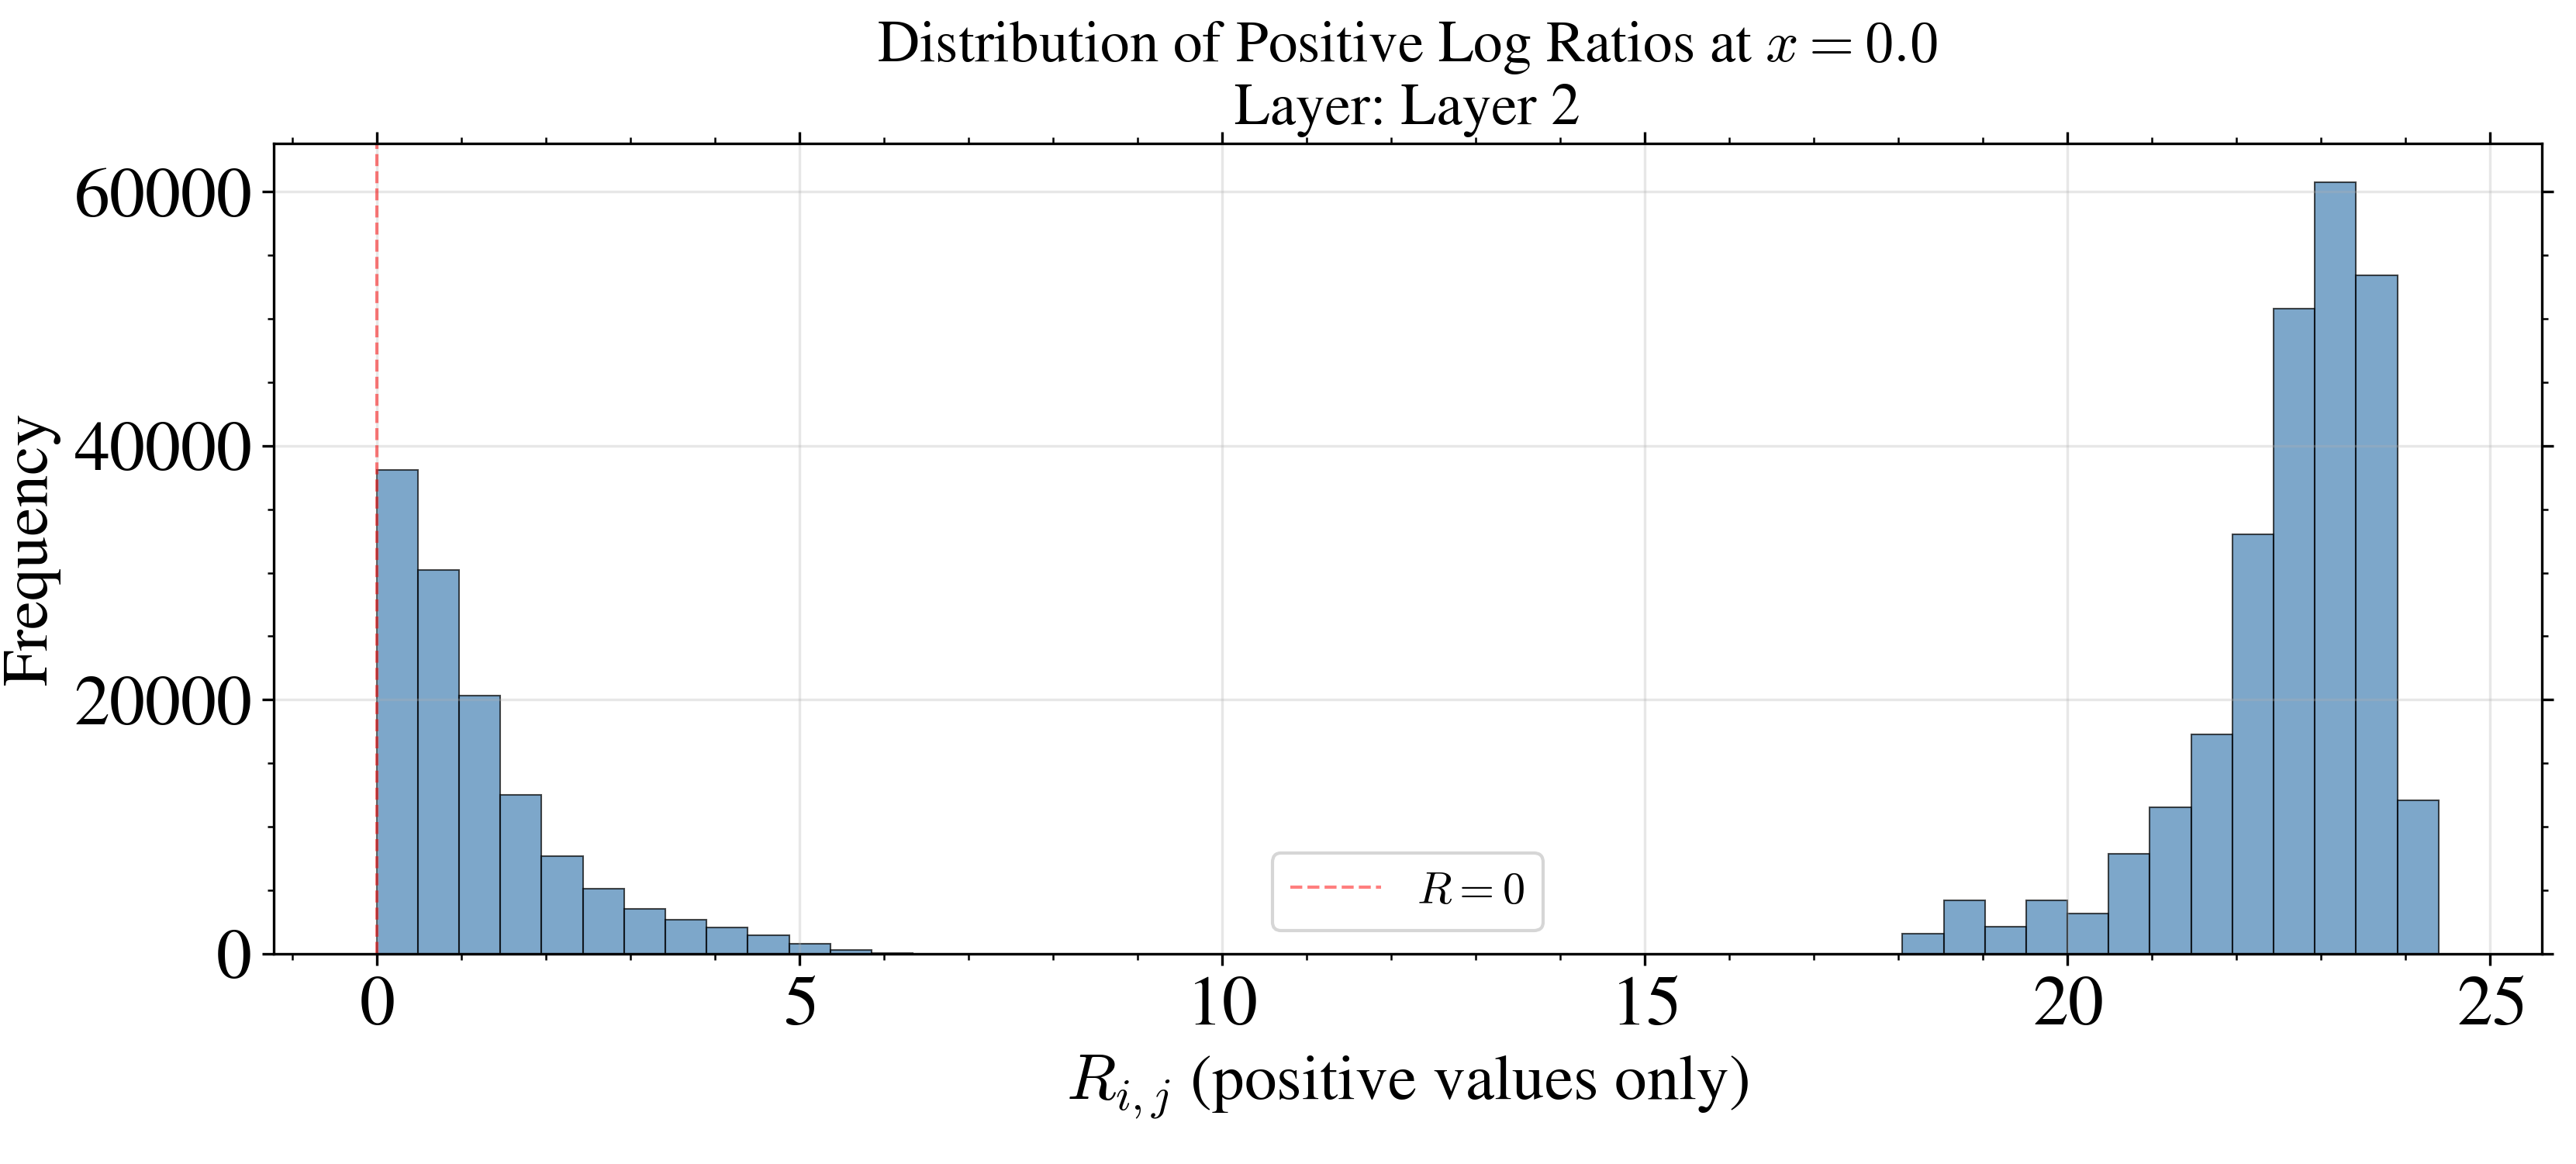
\includegraphics[width=0.5\linewidth]{icml_sgdadamlandscapedynamical/figures/logratio_statistics_x0.png}
\caption{Log-ratios $R_{i,j}$ at $x=0$ over training (all channel pairs).}
\label{fig:logratio-heatmap}
\end{figure}

\begin{figure}[htbp]
\centering
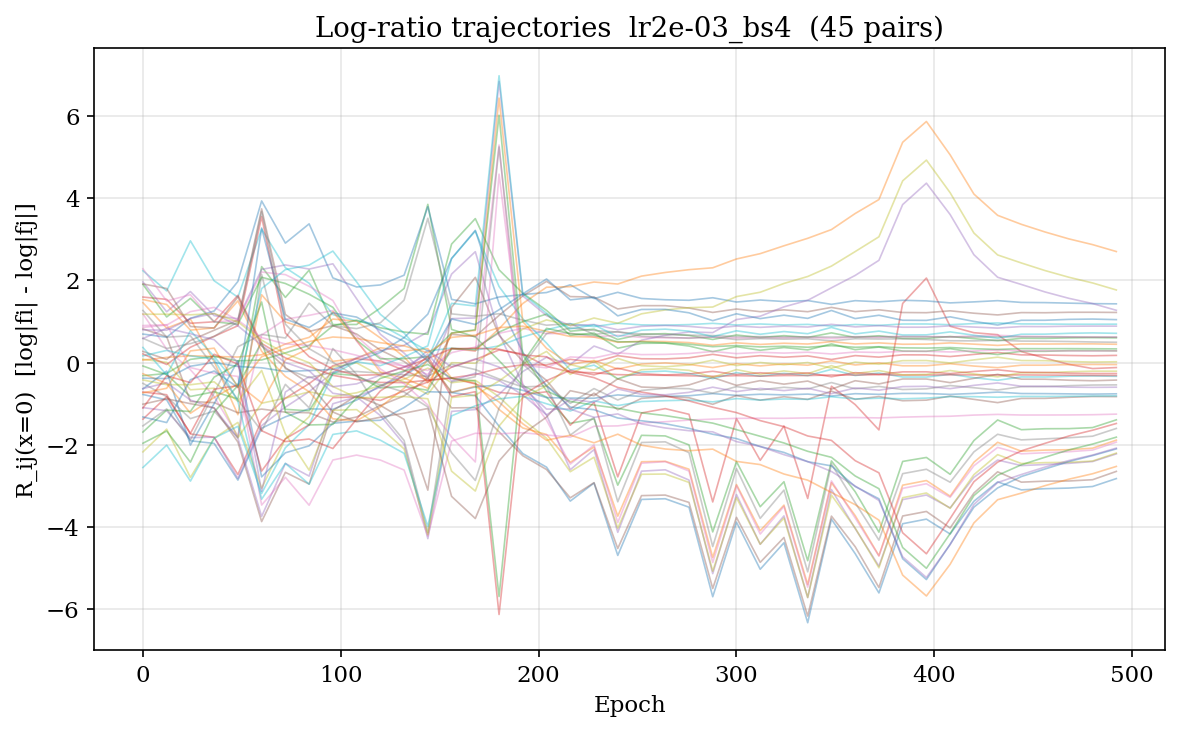
\includegraphics[width=0.42\linewidth]{figures/logratio_trajectories_lr2e-03_bs4_divergence.png}
\caption{Log-ratio trajectories; lr $2{\times}10^{-3}$, bs 4. Divergence by end of training.}
\label{fig:logratio_div}
\end{figure}

\begin{figure}[htbp]
\centering
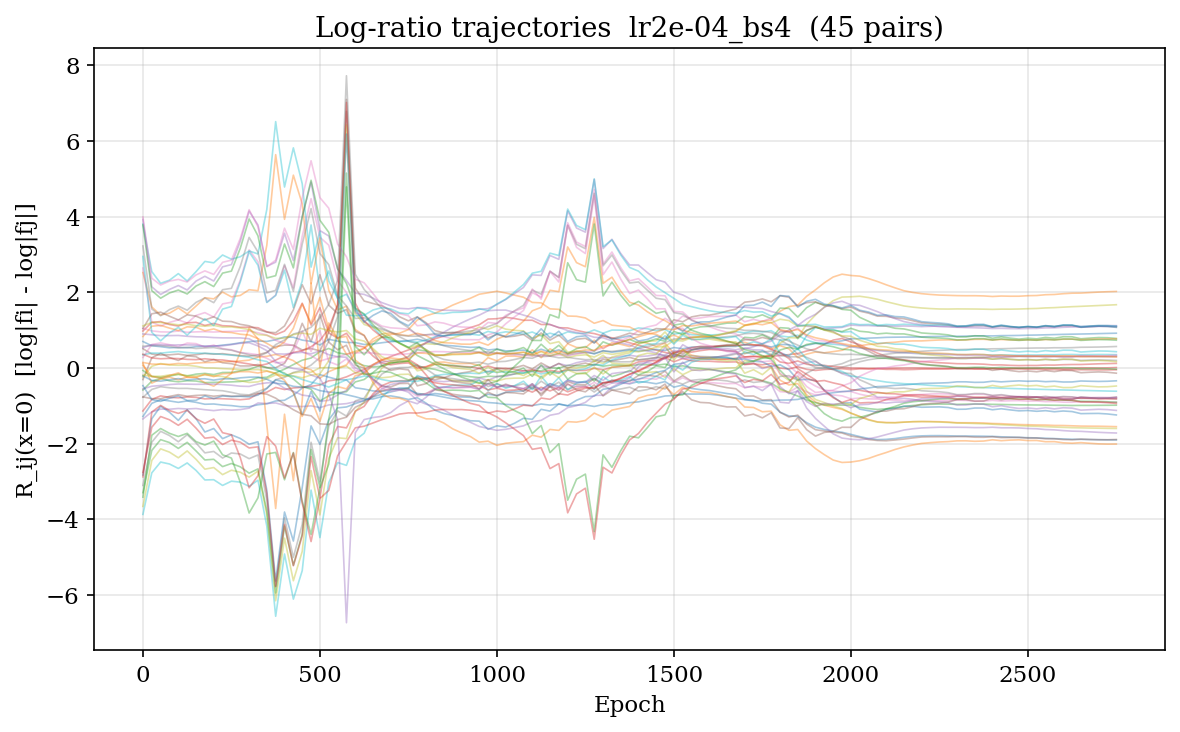
\includegraphics[width=0.42\linewidth]{figures/logratio_trajectories_lr2e-04_bs4_convergence.png}
\caption{Log-ratio trajectories; lr $2{\times}10^{-4}$, bs 4. Convergence (stable specialization).}
\label{fig:logratio_conv}
\end{figure}

\subsection{Oscillatory complexity across layers}
For MMNNs we define the \textbf{mean number of strict local minima per component} $\bar{m}_\ell$ (minima above a small positivity threshold $\varepsilon=10^{-4}$ on a uniform grid). In all runs we observe a \textbf{clear increase in $\bar{m}_\ell$ with layer index $\ell$} in the second half of the network. For $L=6$, $W=128$, early layers (1--4) have $\bar{m}_\ell \le 0.35$; later layers show mean counts from about 1 to 9 (e.g.\ layer 12: $\bar{m}_{12}$ from 2.33 to 8.60 depending on $R$). Distributions are right-skewed. This is consistent with \textbf{deeper layers learning more oscillatory partial functions}. The dependence on rank $R$ is not monotonic in the current single-run-per-config data.

\begin{figure}[htbp]
\centering
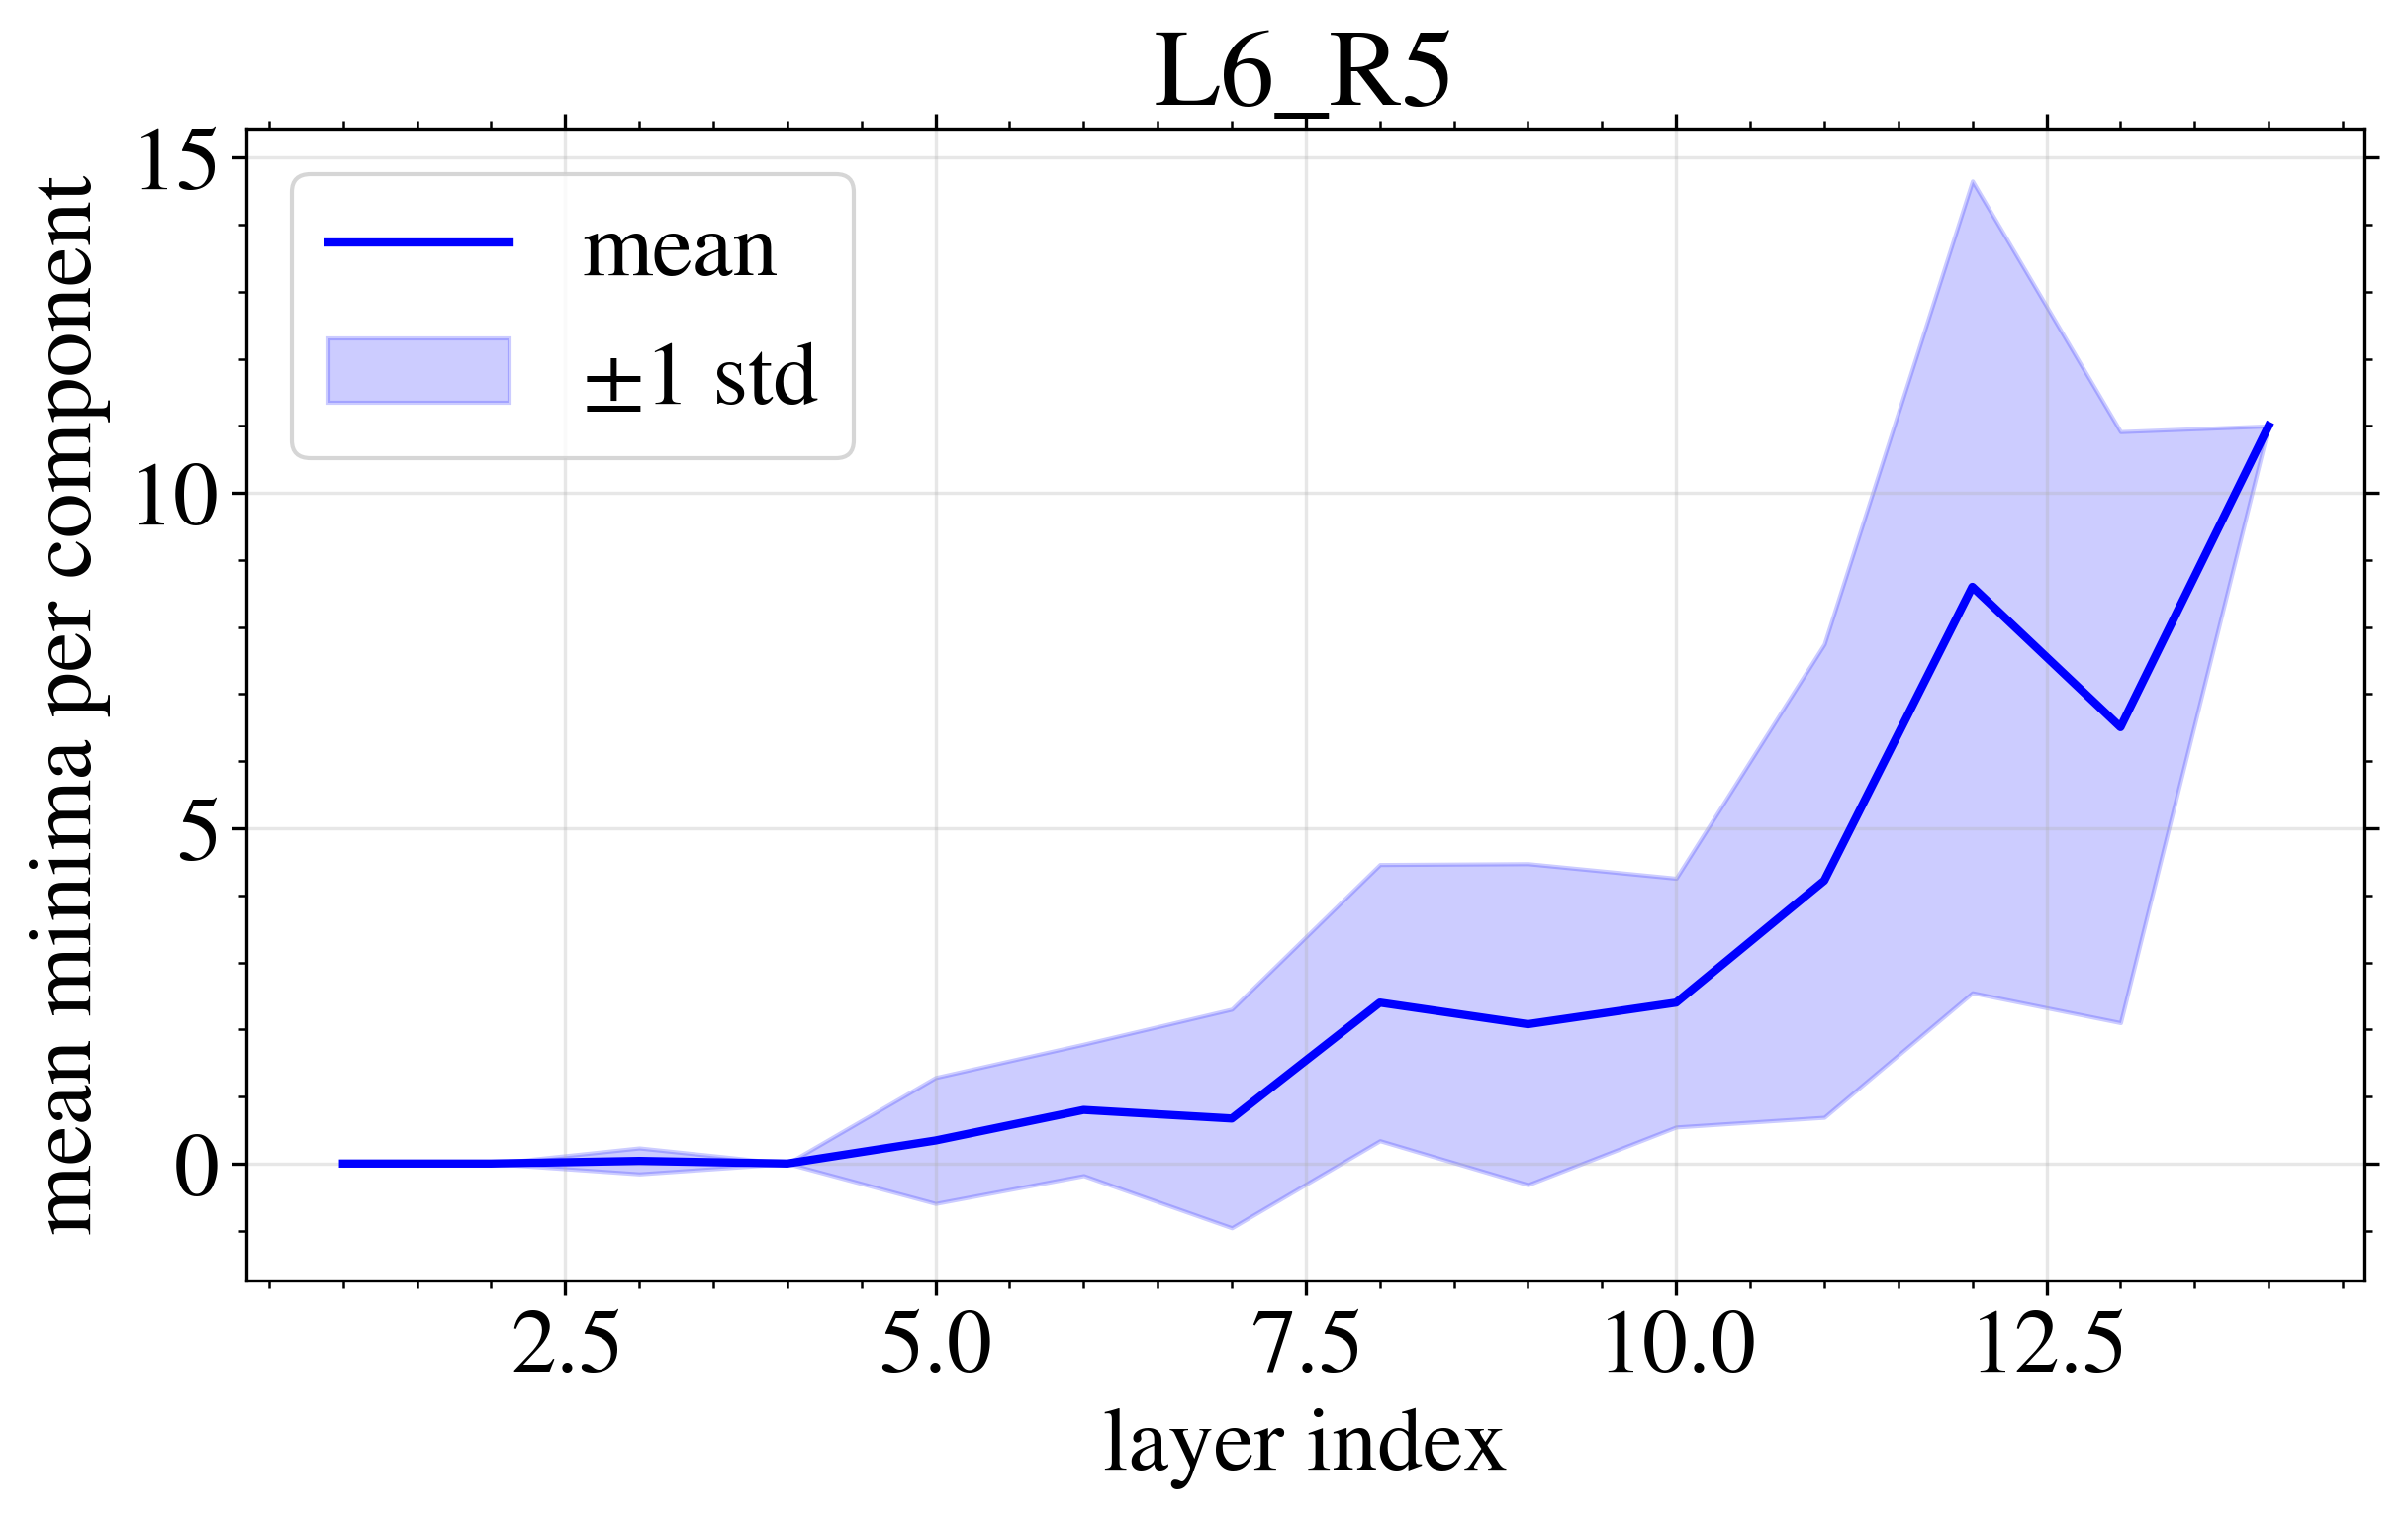
\includegraphics[width=0.5\linewidth]{../../experiments/partialfunctionanalysis/output_leap_all_L6_W128_grouped/grouped/L6_R5/mean_minima_per_component_vs_layer.png}
\caption{Mean number of strictly-positive local minima per component vs.\ layer $\ell$; MMNN $L=6$, $W=128$, $R=5$.}
\label{fig:mean-minima-vs-layer}
\end{figure}

\subsection{Loss, fit, and partials before/after LR reduction}
Figures~\ref{fig:loss_fit_L2} and \ref{fig:loss_fit_L3} show loss and fit before and after LR divides for $L=2$ and $L=3$ (factor $f_3$, $N=768$, bs 8). The sharp loss drops at each LR divide are the empirical signature of sharp basins on a plateau. Figure~\ref{fig:partial_L3} shows partial functions before and after LR divides for $L=3$---the internal representation changes when the trajectory enters a sharper basin.

\begin{figure}[htbp]
\centering
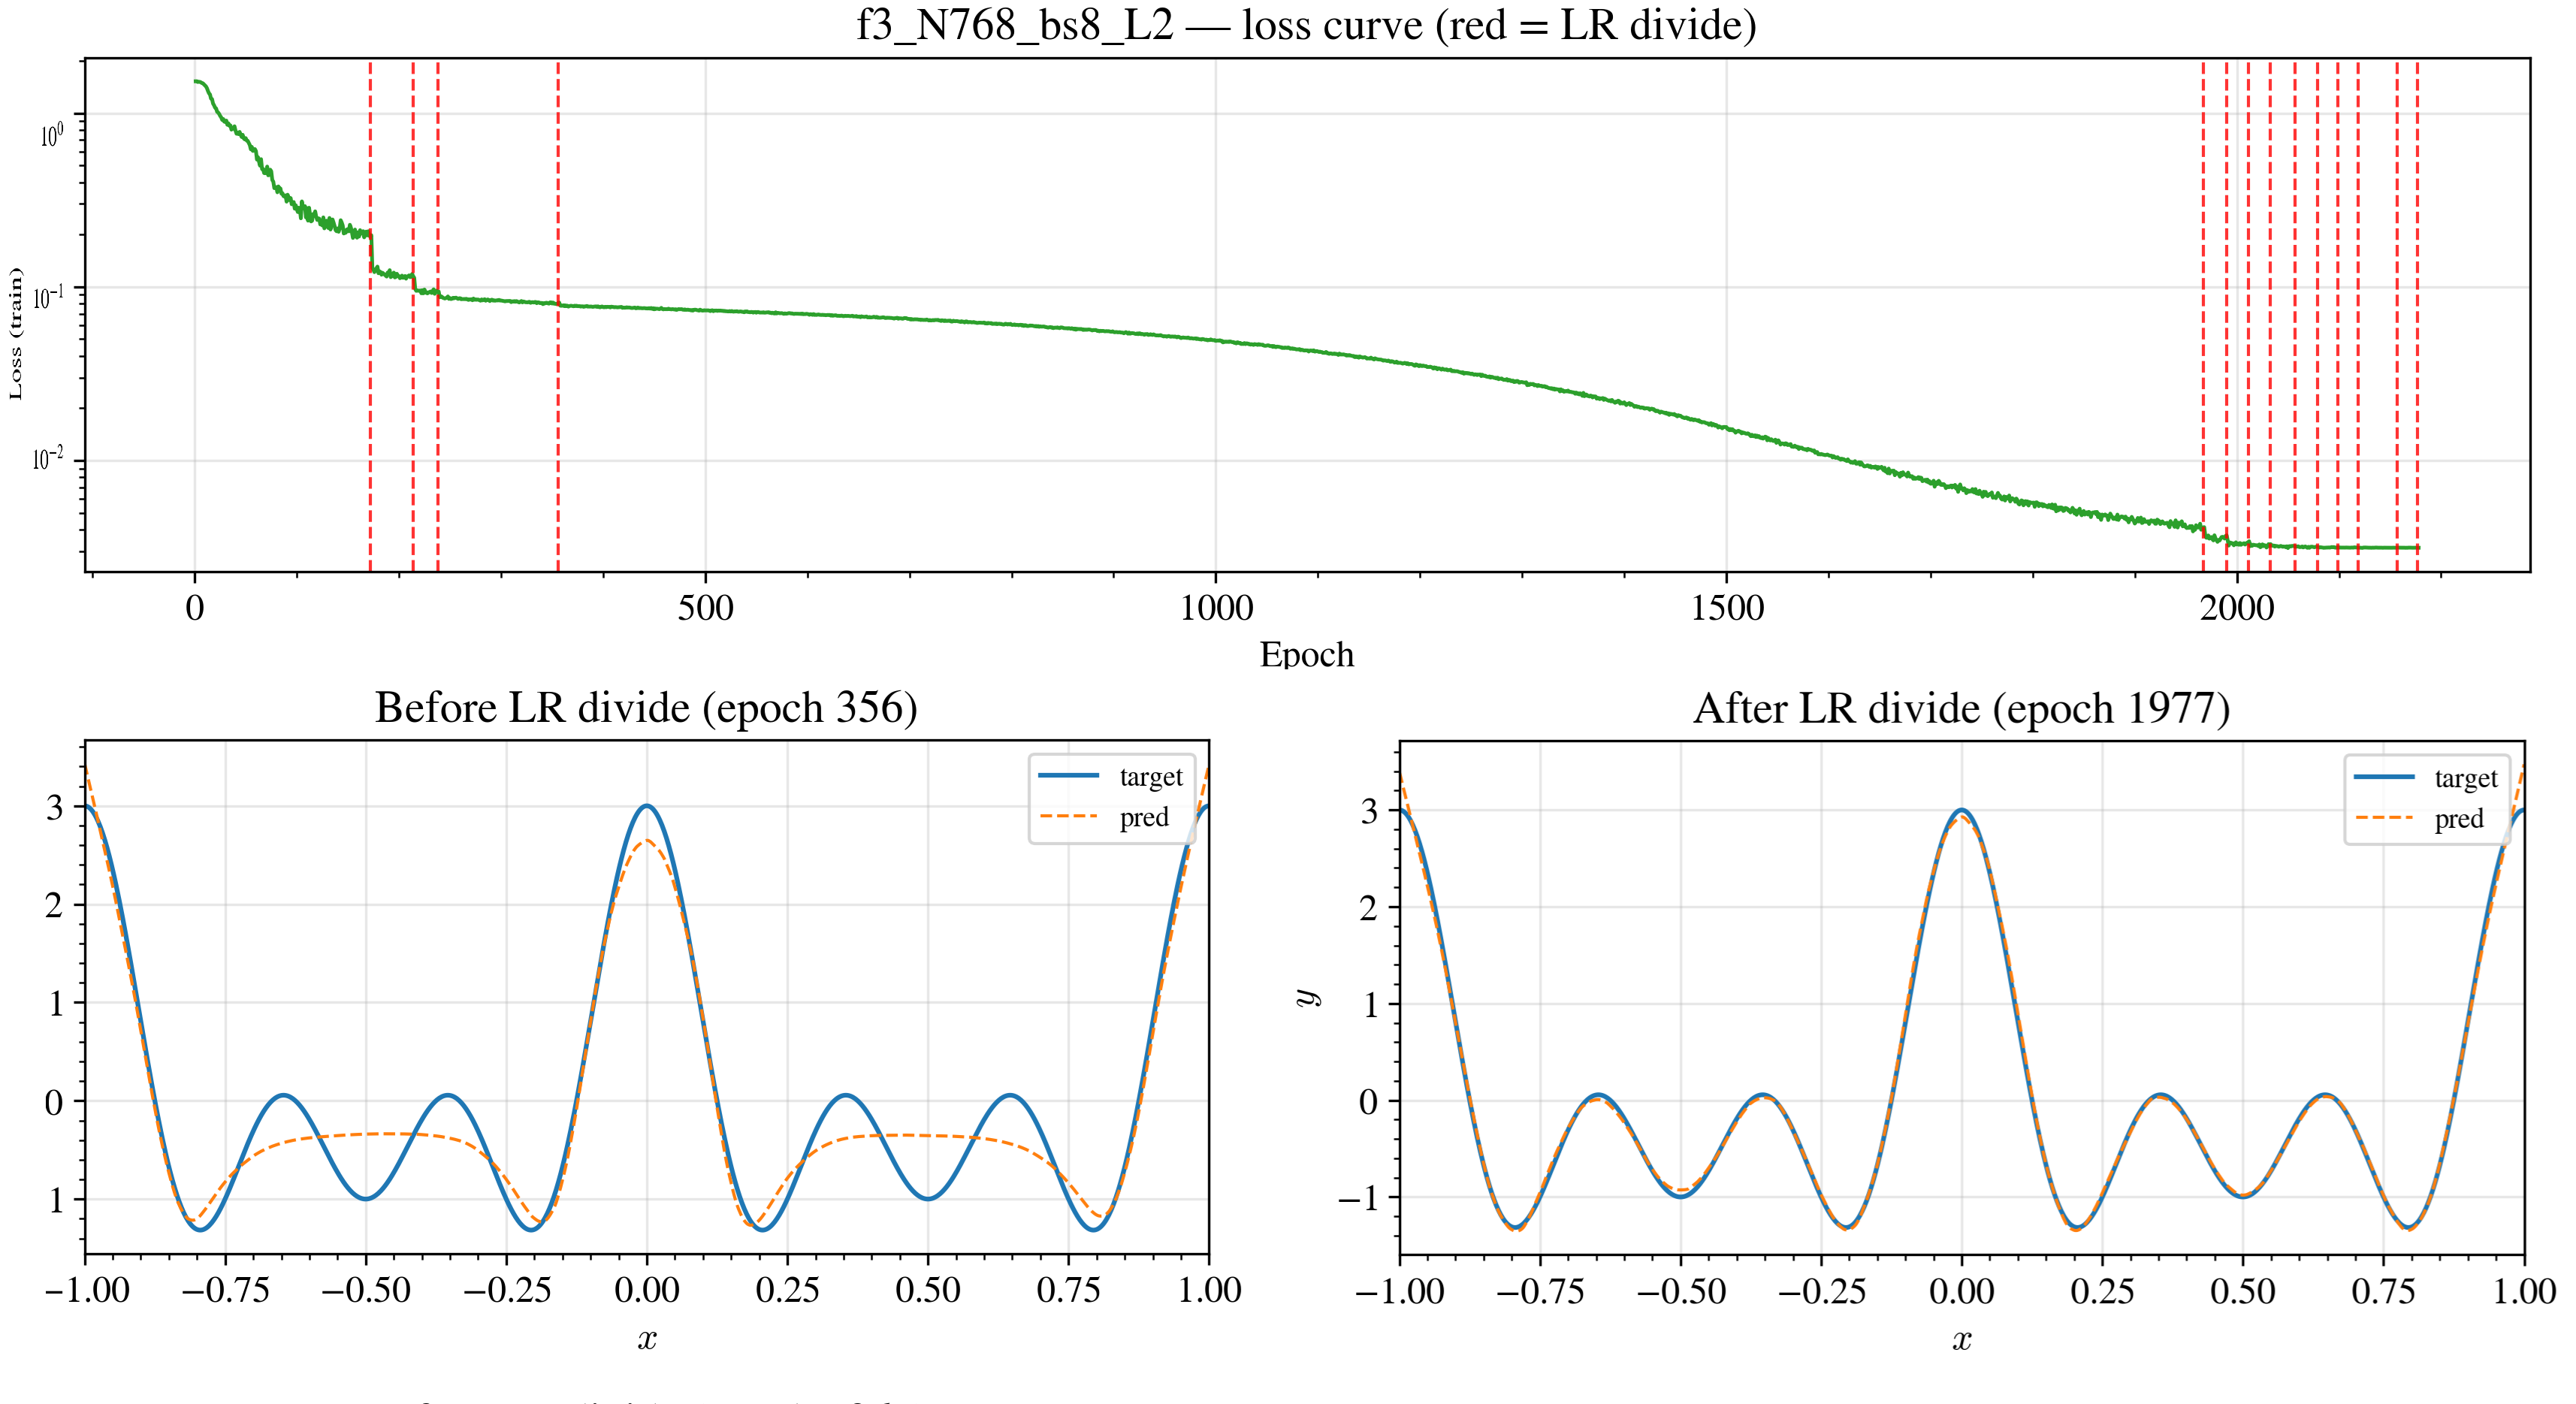
\includegraphics[width=0.42\linewidth]{figures/plot_loss_and_fit_before_after_lr_divides_L2.png}
\caption{Loss and fit before/after LR divides; $f_3$, $N=768$, bs=8, depth $L=2$.}
\label{fig:loss_fit_L2}
\end{figure}

\begin{figure}[htbp]
\centering
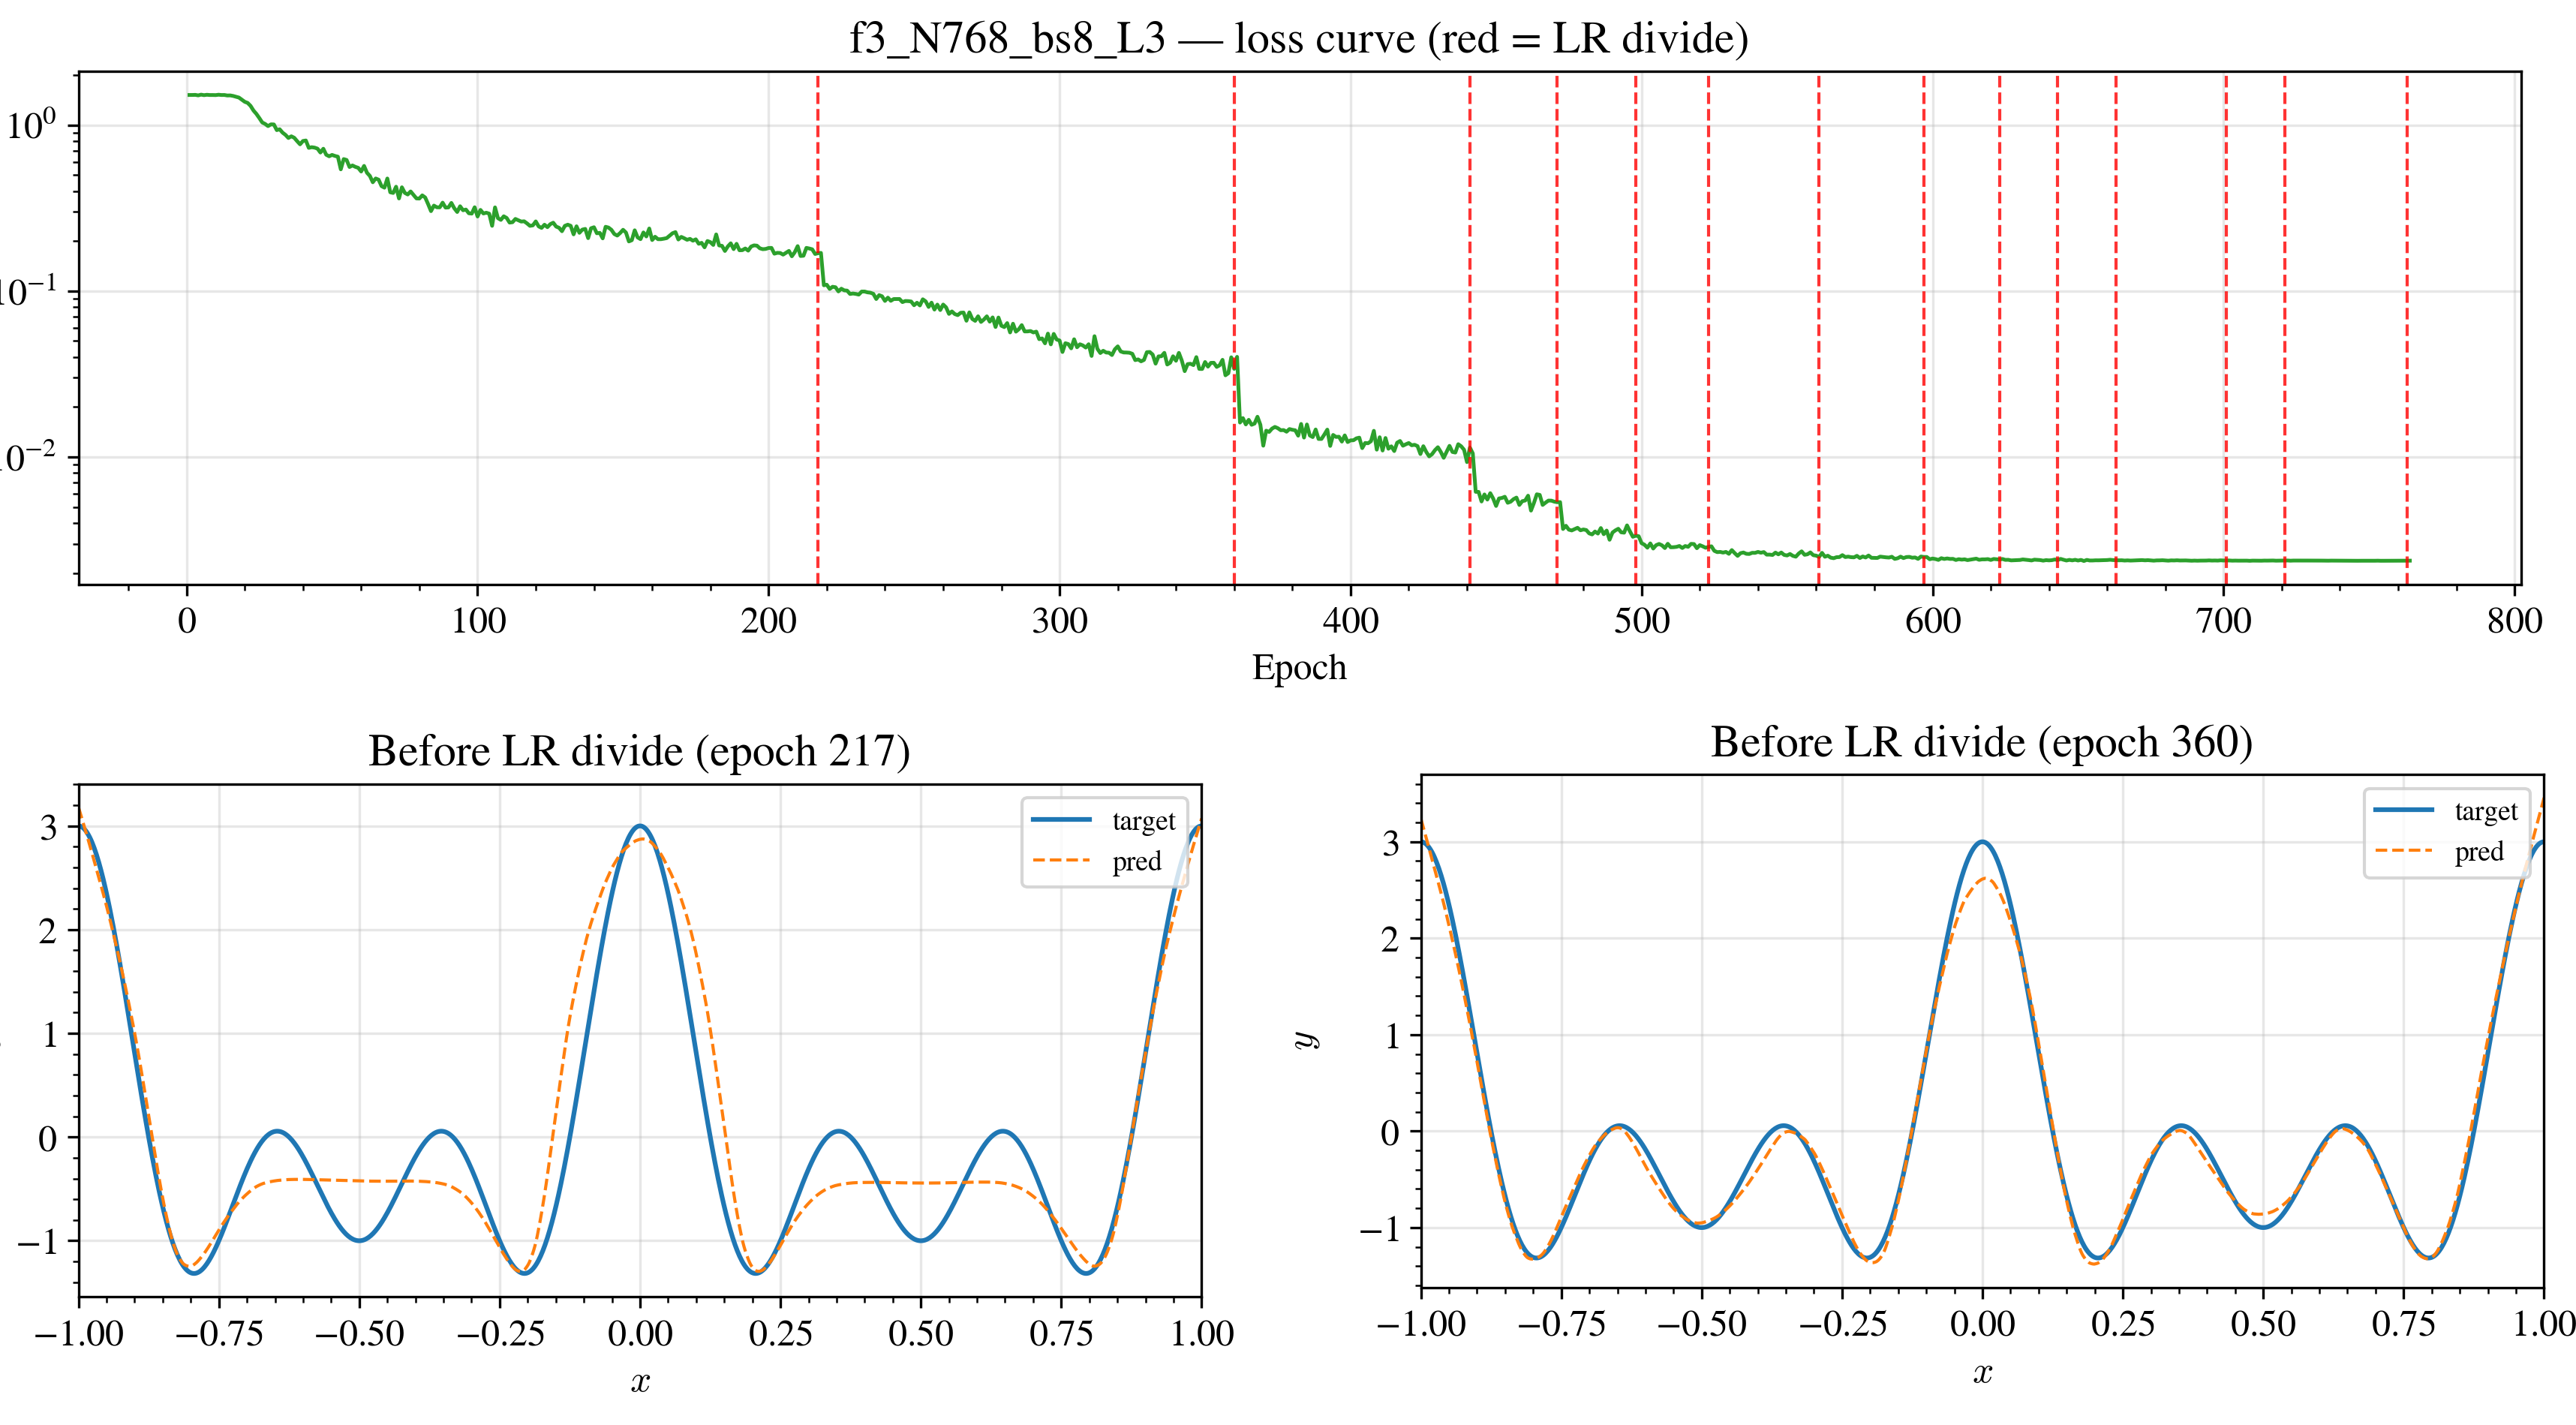
\includegraphics[width=0.42\linewidth]{figures/plot_loss_and_fit_before_after_lr_divides_L3.png}
\caption{Loss and fit before/after LR divides; $f_3$, $N=768$, bs=8, depth $L=3$.}
\label{fig:loss_fit_L3}
\end{figure}

\begin{figure}[htbp]
\centering
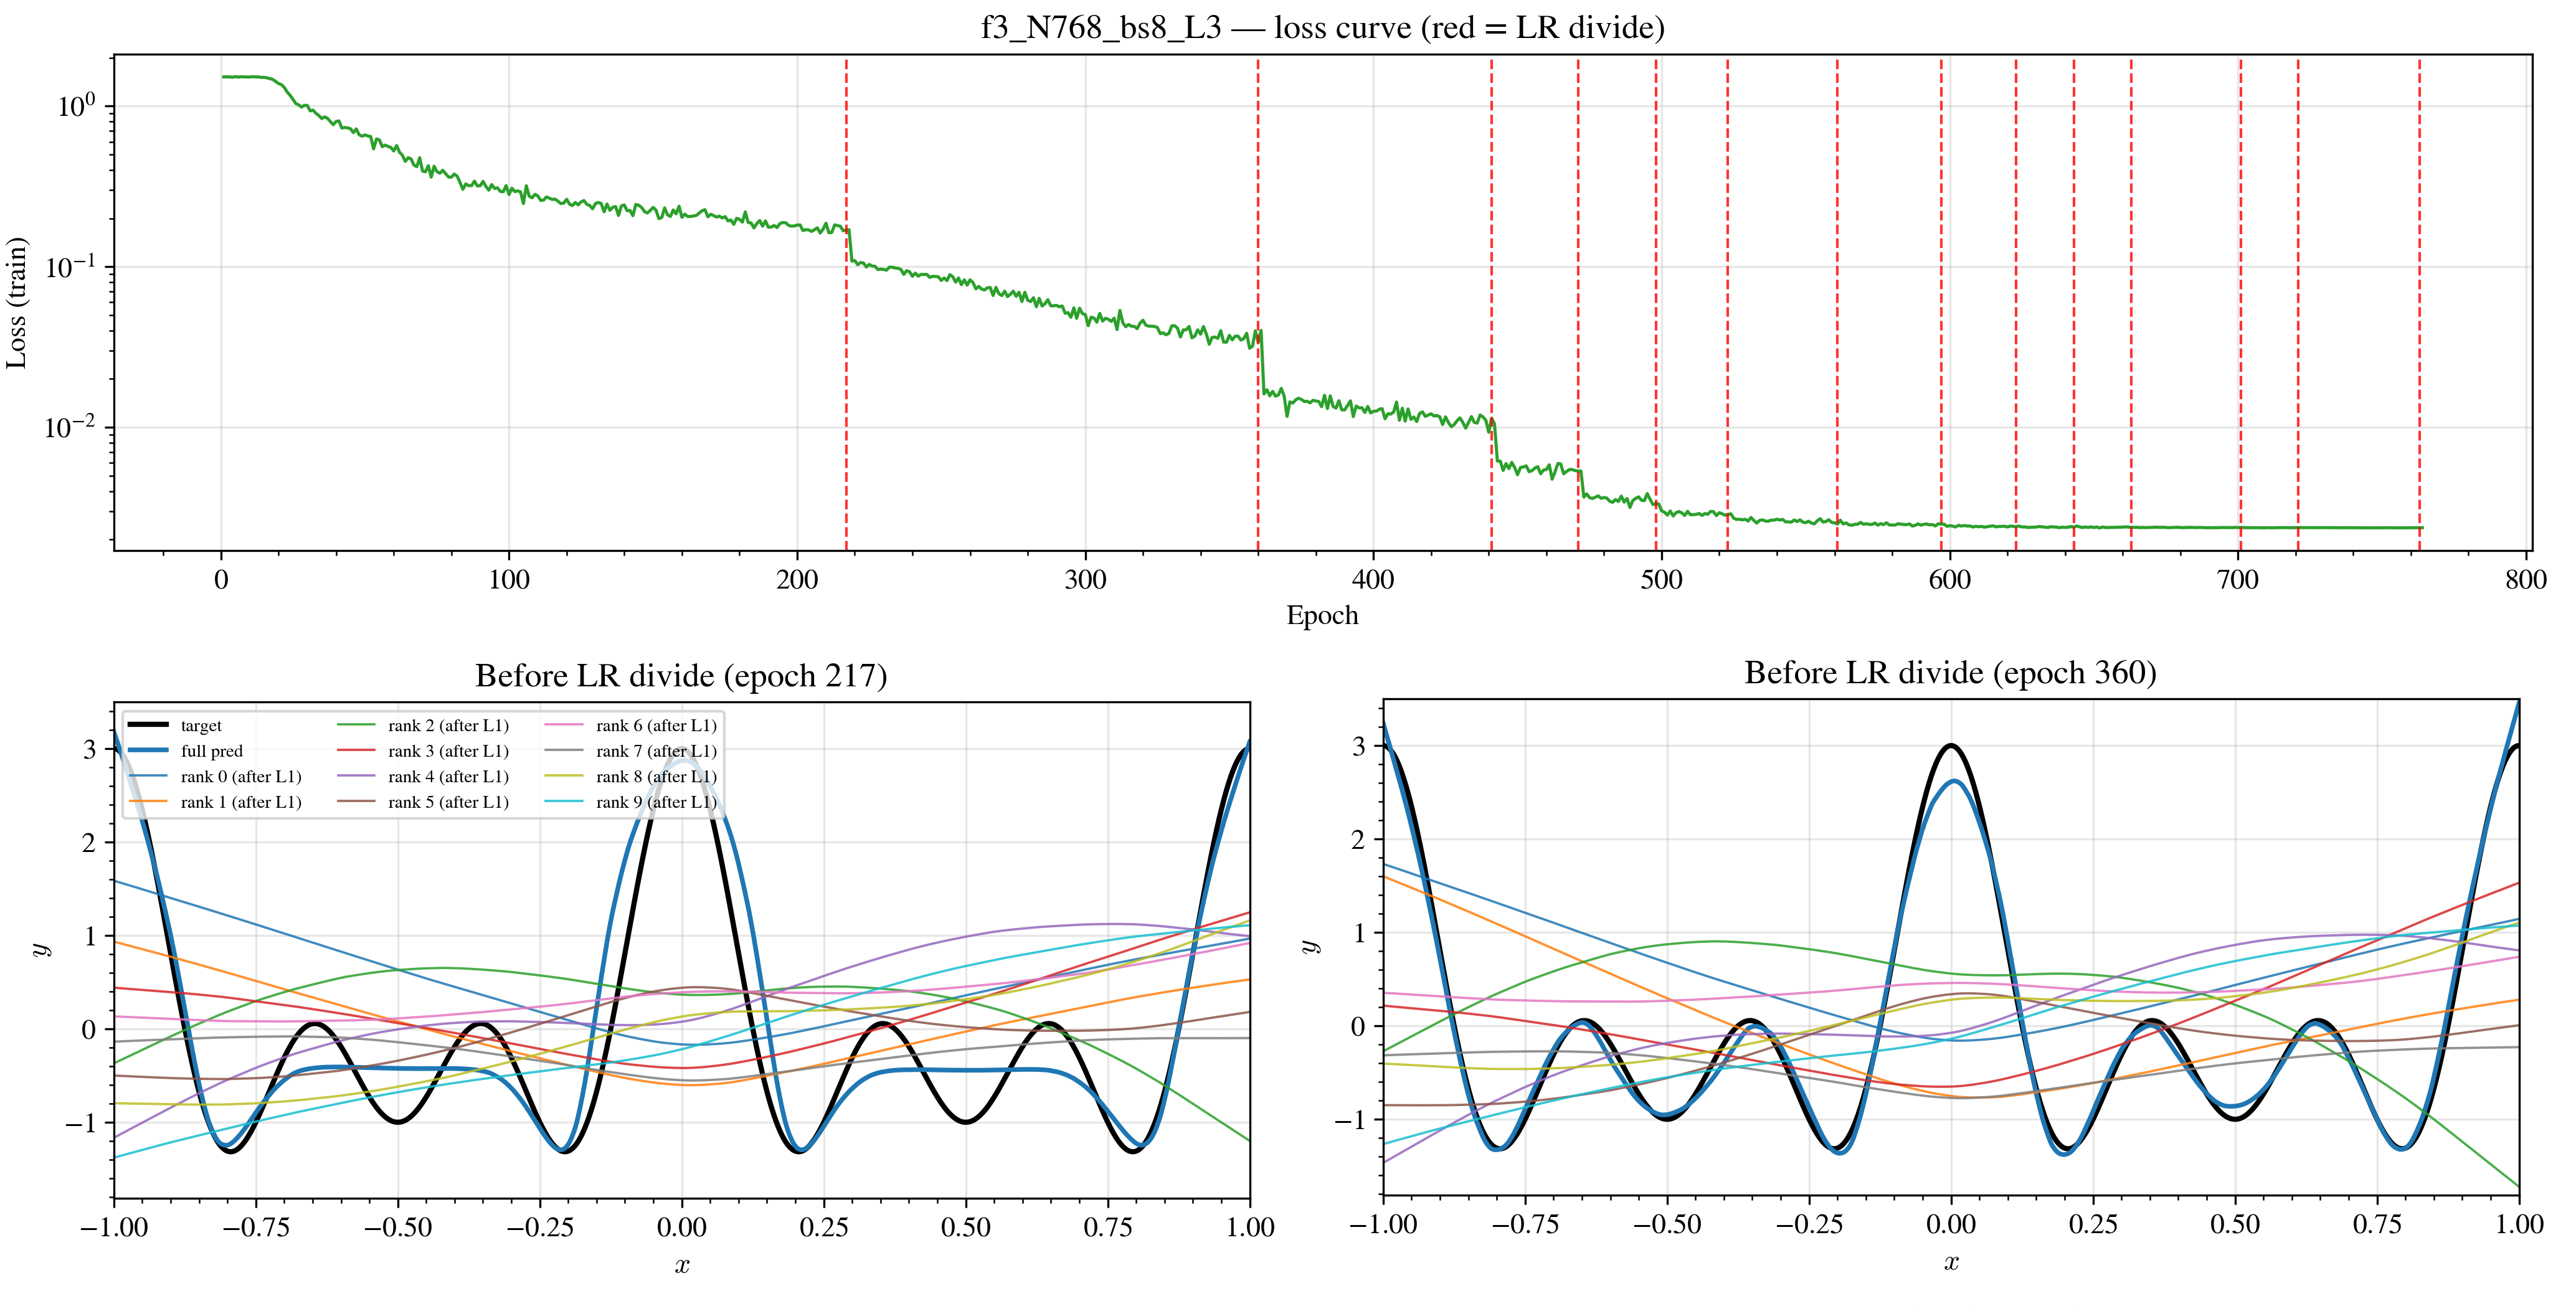
\includegraphics[width=0.42\linewidth]{figures/plot_partial_before_after_lr_divides_L3.png}
\caption{Partial functions before/after LR divides; $f_3$, $N=768$, bs=8, depth $L=3$.}
\label{fig:partial_L3}
\end{figure}

\section{Adam, symmetry preservation, and scaling}
\label{sec:adam-scaling}

\subsection{Adam and instability}
In our setting, Adam is observed to be highly unstable. A jump near end-of-schedule (EOS) can sometimes land the solution in a sharp basin. The lower part of the landscape appears more sensitive to $N$ than the upper part.

\subsection{Symmetry preservation: low-rank vs full-rank}
Targets such as $y(x)=\sum_k \cos(2\pi k x)$ or $f(x)=\cos(f_1\pi x^2)-0.8\cos(f_2\pi x^2)$ on $[-1,1]$ are \textbf{symmetric about $x=0$}. Under batched optimization, full-rank (MLP) networks can learn \emph{asymmetric} internal representations; low-rank (RF-LR or MMNN) networks tend to \textbf{preserve symmetry} in the channel partials. Figure~\ref{fig:mlp-asymmetry} shows the asymmetry when RF/low-rank is removed: at layers 7 and 16 the learned features are visibly asymmetric about $x=0$ (same setup as symmetric low-rank: 8 layers, $n=1024$, $r=20$, target $(f_1,f_2)=(144,48)$, $N=4k$, Adam, batch 100). The low-rank constraint acts as an implicit regularizer that preserves the target's symmetry.

\begin{figure}[htbp]
\centering
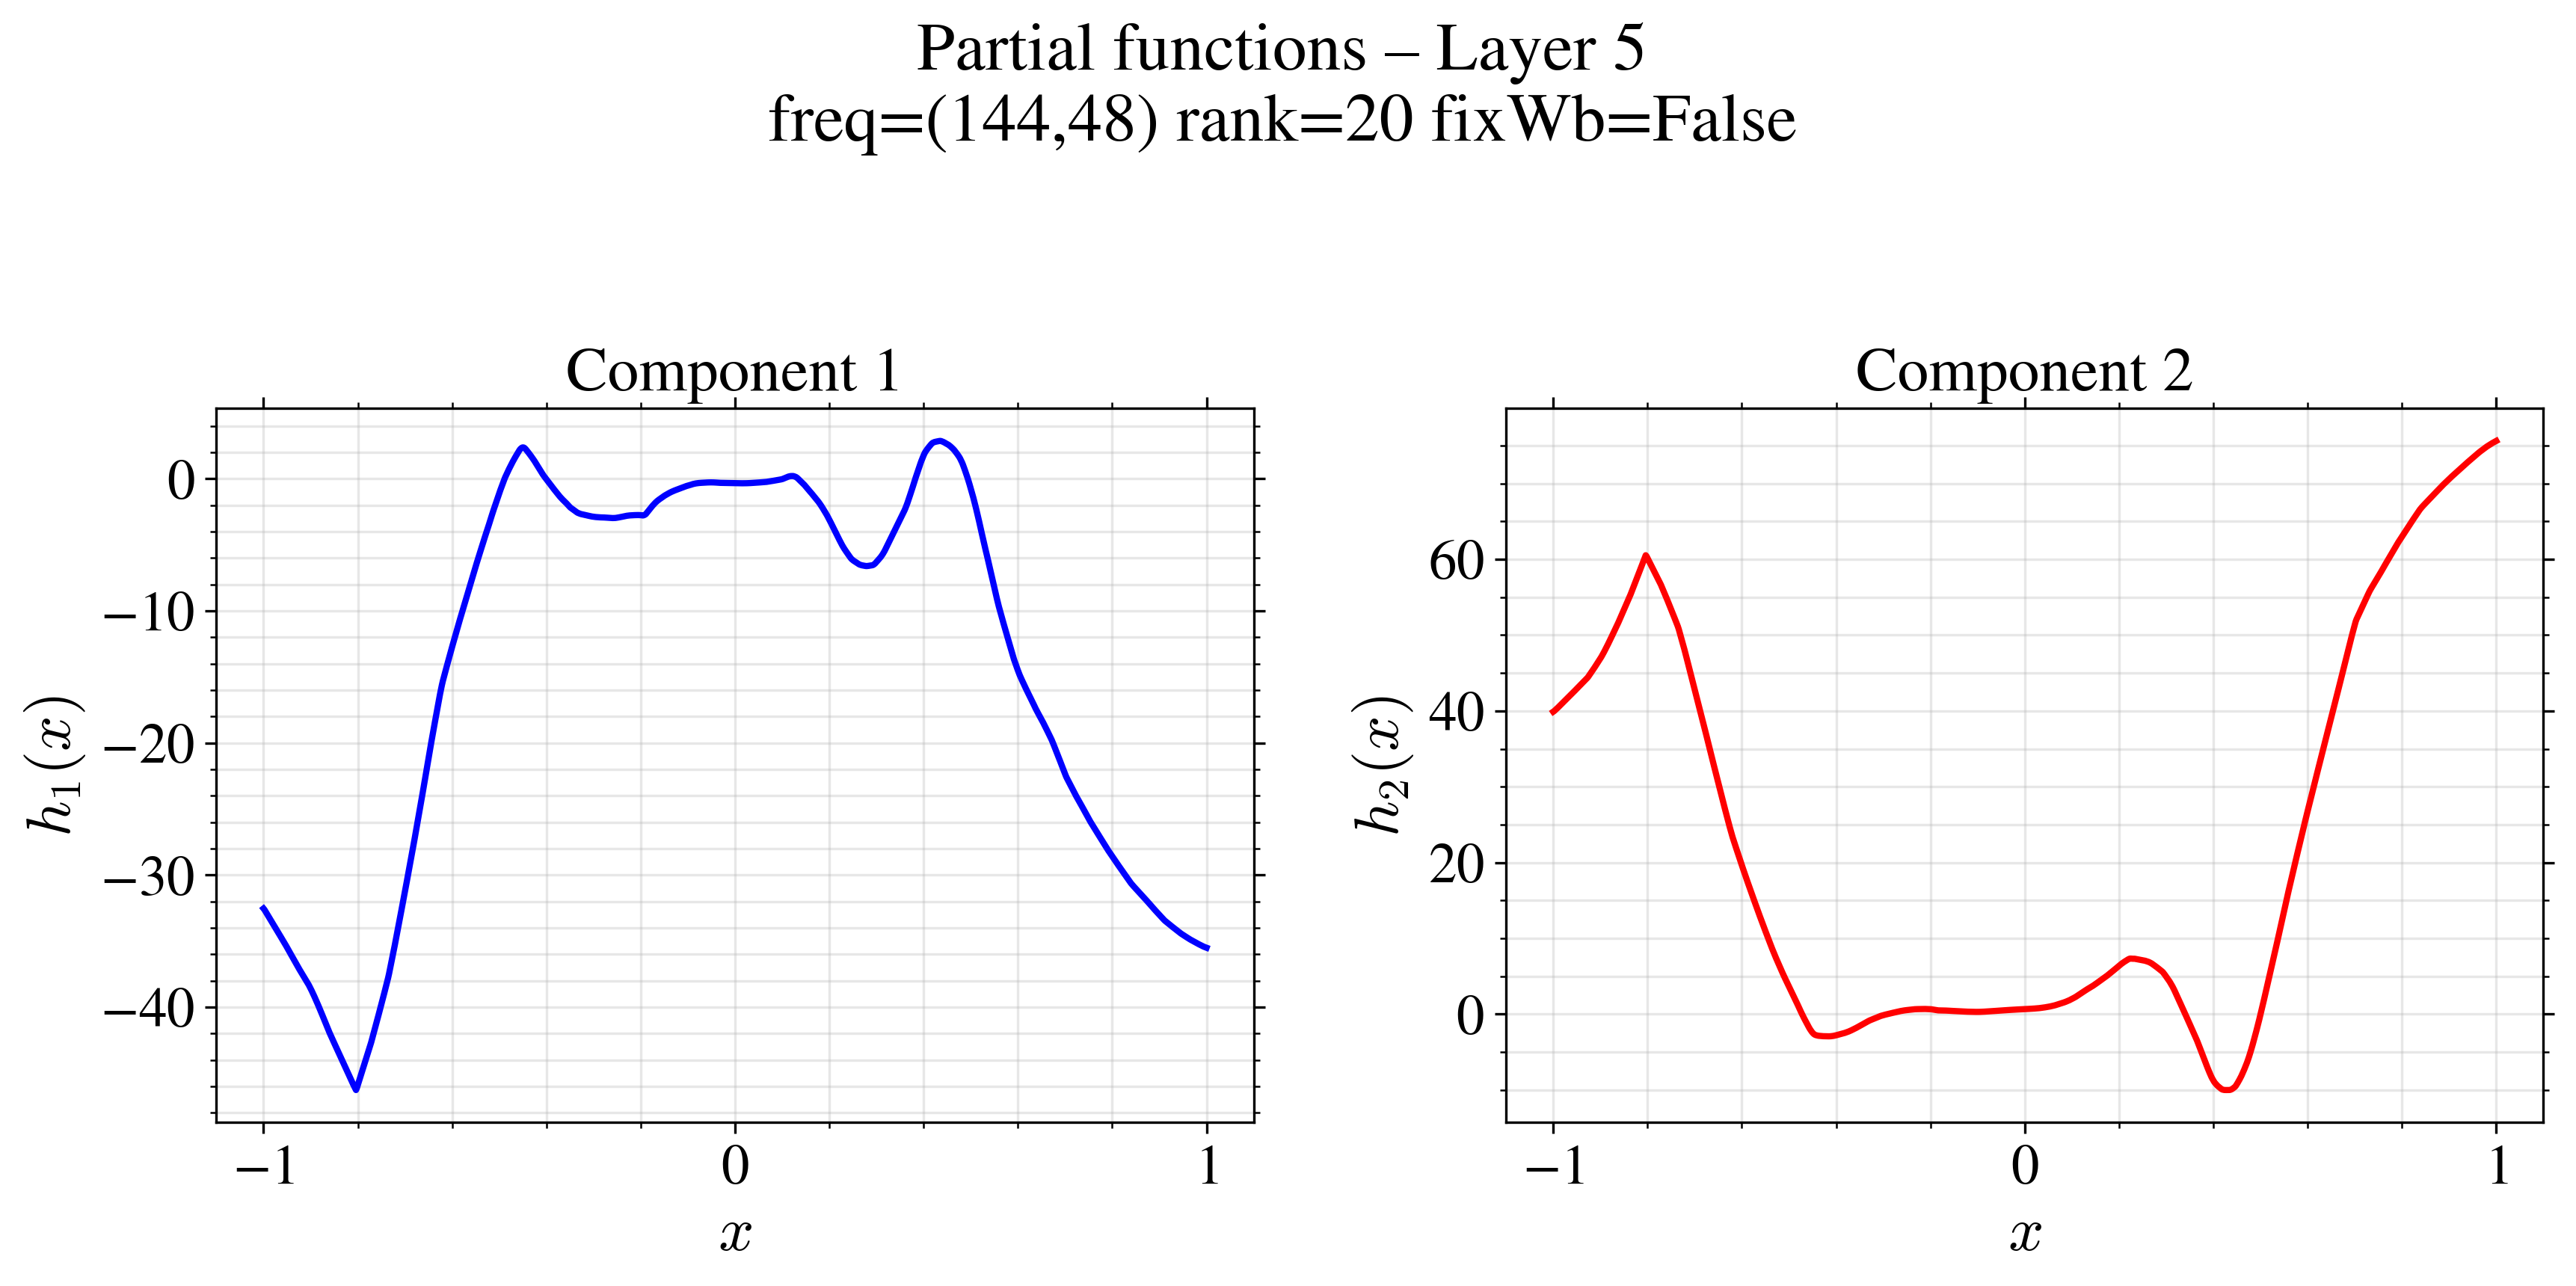
\includegraphics[width=0.42\linewidth]{figures/mlp_asymmetry_layer7.png}\hfill
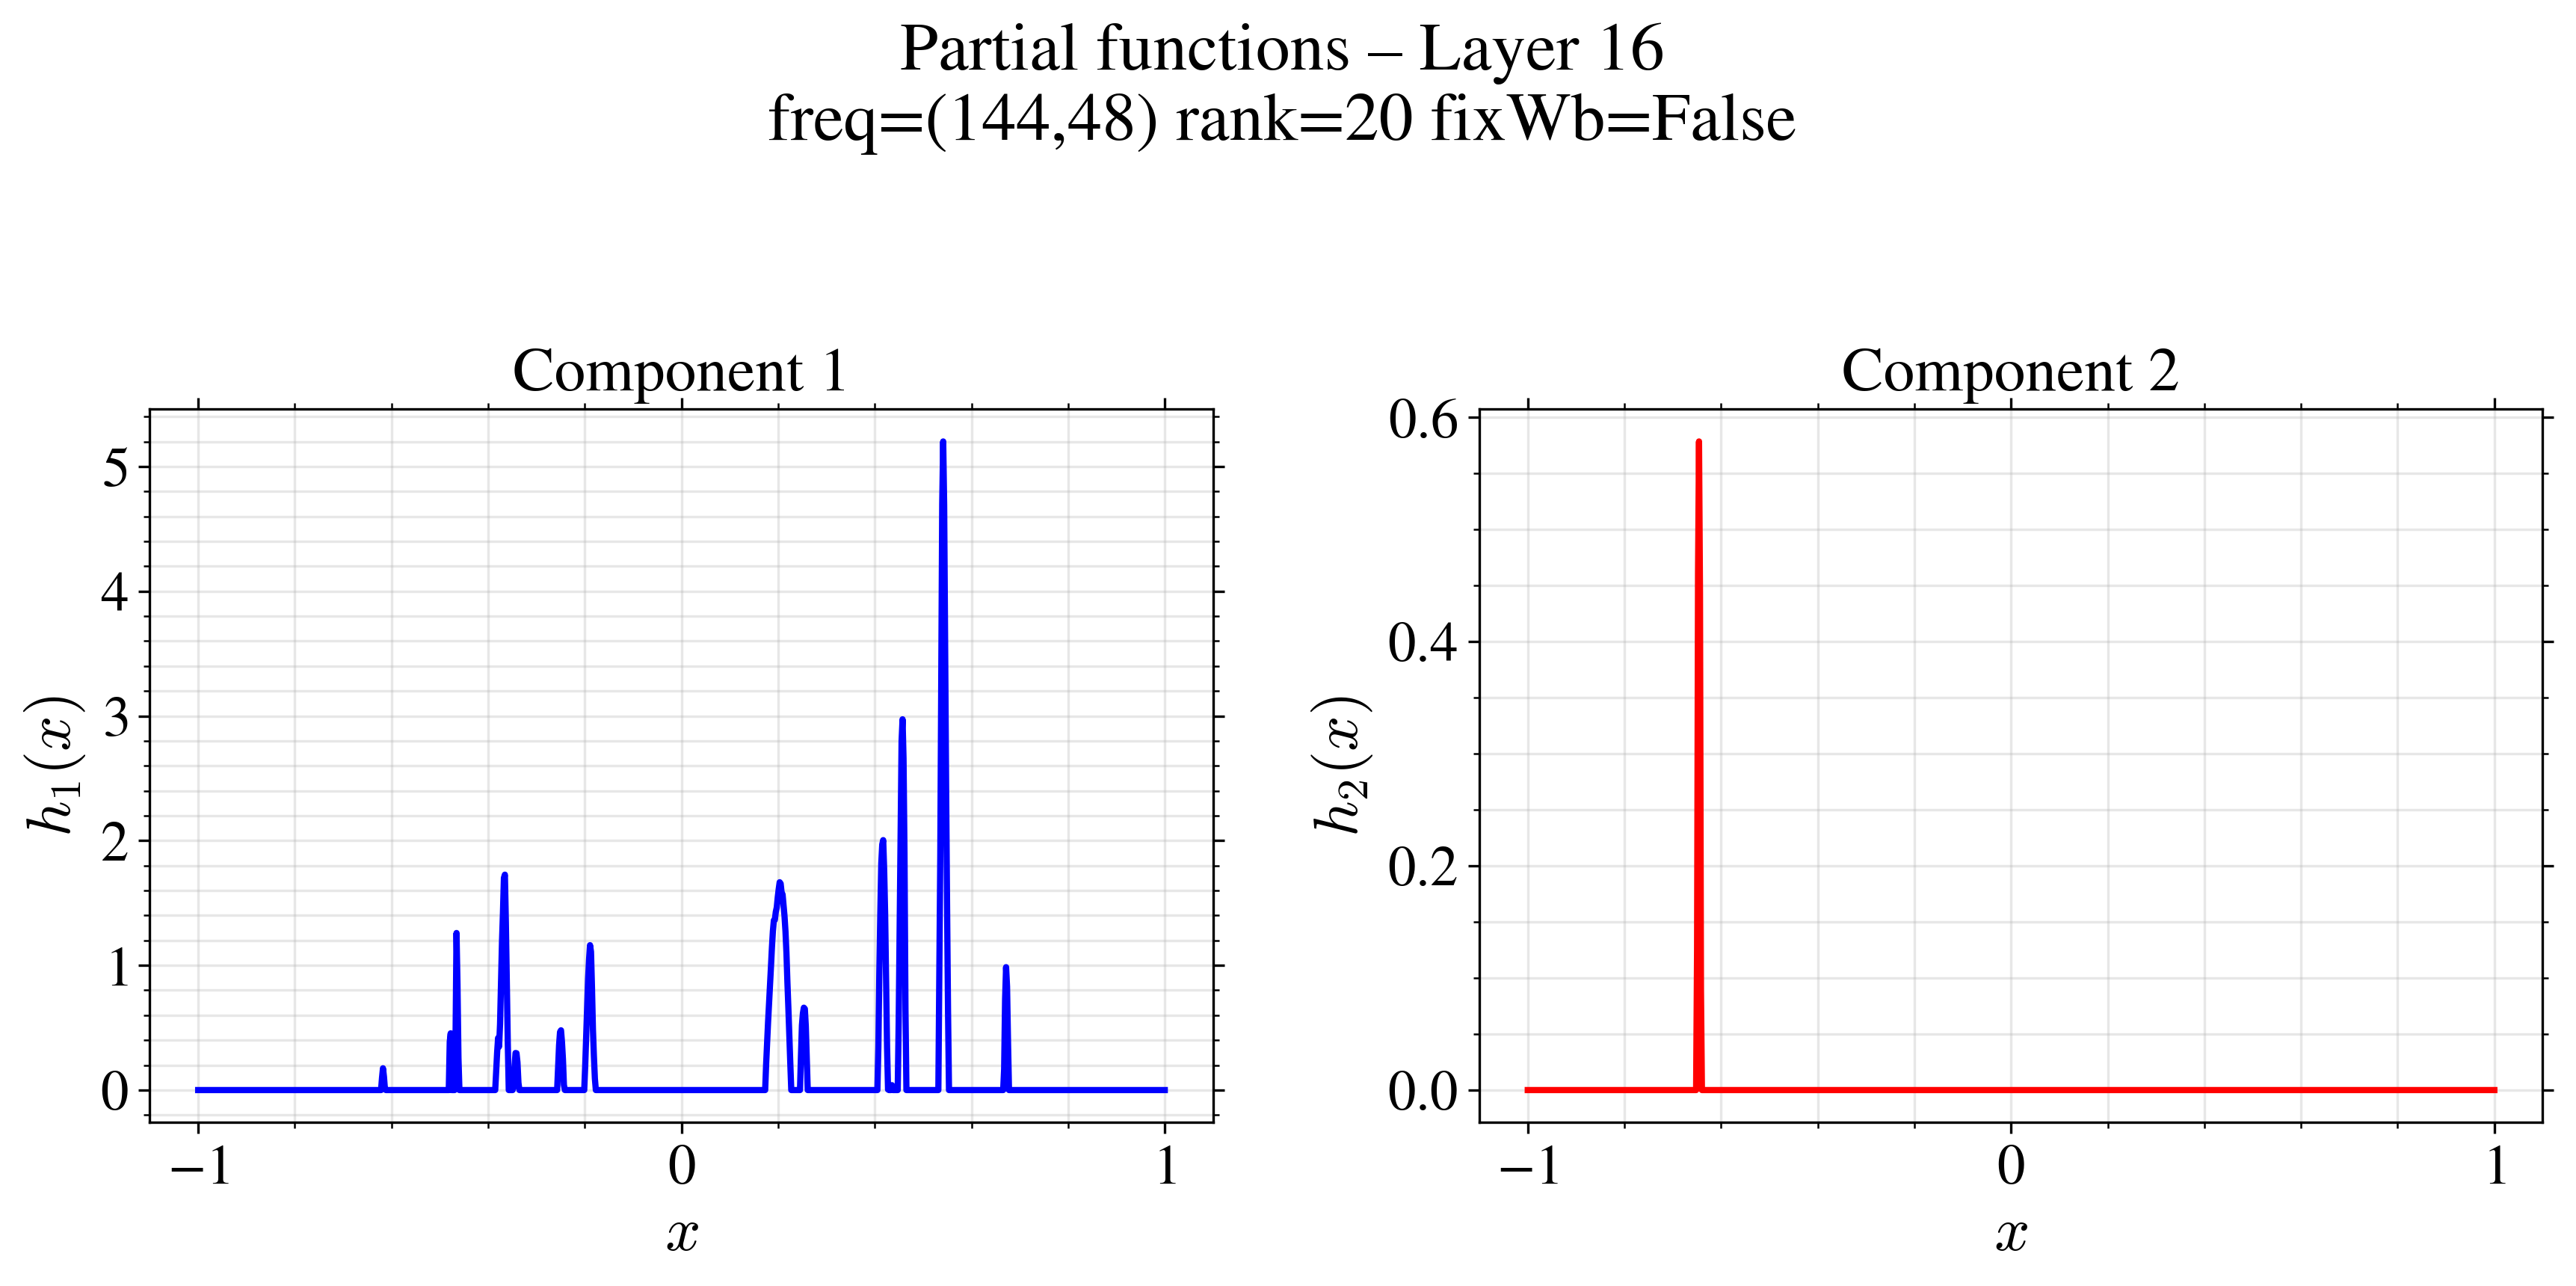
\includegraphics[width=0.42\linewidth]{figures/mlp_asymmetry_layer16.png}
\caption{Symmetry comparison: full-rank MLP (RF removed) learns asymmetric features at layers 7 and 16 despite symmetric target; low-rank preserves symmetry.}
\label{fig:mlp-asymmetry}
\end{figure}

\subsection{Scaling}
\textbf{Plateau-escape time} scales roughly like $1/\mathrm{lr}$ (e.g.\ $\sim$20 epochs for lr $10^{-2}$ vs.\ $\sim$2000 for lr $10^{-4}$), with dependence on batch size (small batch 1--4 escapes effectively). Figures~\ref{fig:escape_vs_lr} and \ref{fig:escape_vs_bs} show epochs to escape vs.\ LR and vs.\ batch size. Layer $L$ can exhibit on the order of $2L$ spikes in the partial functions, a distinctive feature-learning signature. Very deep nets ($L=56$, 80) can exhibit blow-up or NaN in frequency/layer-scaling runs.

\begin{figure}[htbp]
\centering
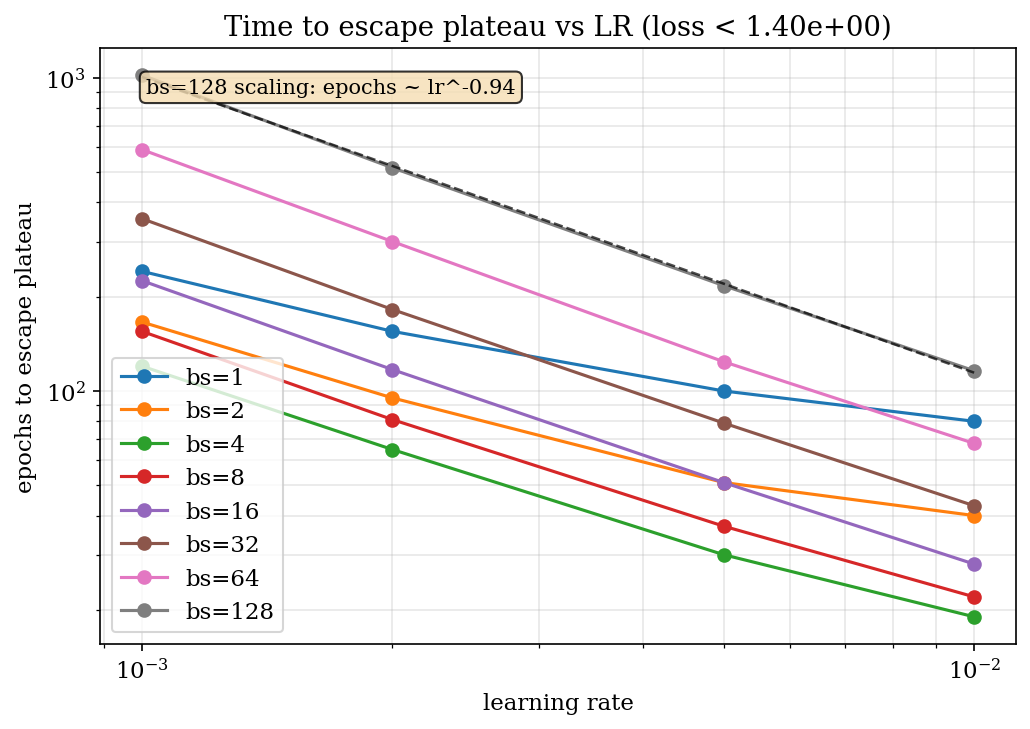
\includegraphics[width=0.42\linewidth]{figures/epochs_to_escape_vs_lr.png}
\caption{Epochs to escape the first plateau vs.\ learning rate.}
\label{fig:escape_vs_lr}
\end{figure}

\begin{figure}[htbp]
\centering
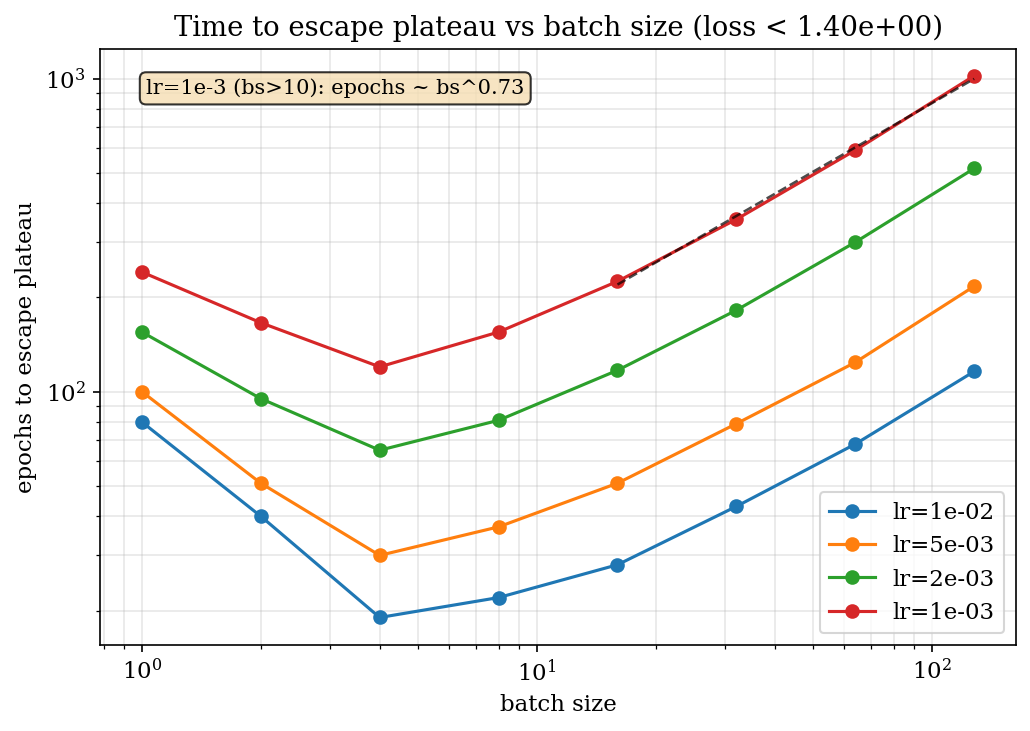
\includegraphics[width=0.42\linewidth]{figures/epochs_to_escape_vs_bs.png}
\caption{Epochs to escape vs.\ batch size. Small batch (1--4) escapes effectively.}
\label{fig:escape_vs_bs}
\end{figure}

\section{Limitations}
\label{sec:limitations}

This study is restricted to 1D regression with the sum-of-cosines (and related) target and the MMNN/RF-LR architecture; we do not claim that the same feature--landscape relation holds in higher dimensions or for other architectures without further experiments. Observations on Adam and on self-similarity of training curves are qualitative; replication over seeds and hyperparameters would be needed for robust scaling statements. Oscillatory-complexity results are from single runs per config; the minima count is a lower bound (grid resolution). Very deep networks can become unstable (stability frontier). The reported configs and script index in the Appendix are intended to make the methodology reproducible.

\section{Conclusion}
\label{sec:conclusion}

We presented a \textbf{unified picture} of feature learning and the loss landscape for low-rank neural networks in a controlled 1D setting. The log-ratio criterion and two-sided step toy model formalize when channel dominance is maintained; log-ratio trajectories and oscillatory-complexity statistics (mean minima per component) provide empirical support. The loss exhibits a plateau--sharp--plateau structure aligned with frequency learning; the landscape is a plateau with sharp, deep basins that become accessible when the learning rate is small; and observables such as mean minima per component and the $2L$-spike pattern per layer $L$ bridge landscape and feature learning. Low-rank structure also preserves the target's geometric symmetry while full-rank nets can break it. Within the stated scope, understanding the loss landscape in these networks amounts to understanding how and when features are acquired. These observations support the SciForDL goal of building a scientific understanding of deep learning through reproducible experiments and explicit reporting of the relation between landscape geometry and learned representations.

\bibliography{iclr2026_conference}
\bibliographystyle{iclr2026_conference}

\appendix
\section{Full experiment methodology and configs (exhaustive)}
\label{app:methodology}

All paths and commands below are relative to repo root \texttt{MMNN/} unless noted. Full reference: \texttt{experiments/table/EXHAUSTIVE\_RESULTS\_BASELINE\_SWEEP\_RANKS.md}, \texttt{INDEX\_LOGRATIO\_ESCAPE\_SCALING.md}, \texttt{BASELINE\_SWEEP\_SETUPS\_AND\_RANKS.md}.

\subsection{Target and architecture (all experiments)}
Target: $y(x) = \sum_{k=1}^{\mathrm{factor}} \cos(2\pi k x)$ on $x \in [-1,1]$. MMNN: input/output dim 1; hidden rank $R$, width $W$; depth $L$ blocks (linear rank$\to$width, ReLU, linear width$\to$rank). fixWb = True. $\mu$-parameterization; SGD momentum 0; gradient clipping max norm 1.0.

\subsection{Main figures (loss, fit, partials)}
Factor 3, $N_{\mathrm{train}}=768$, batch 8, depths $L=2,3$. Configs \texttt{f3\_N768\_bs8\_L2}, \texttt{f3\_N768\_bs8\_L3}. Architecture: width 1024, rank 10. Training: num\_epochs 10,000; lr initial 0.01, divide by 2 on stagnation (25 steps); lr\_window 10, min\_epochs\_before\_reduce 20. Checkpoints: before and 10 epochs after each LR divide.

\subsection{Baseline sweep: commands and sweep definition}
\label{app:baseline-sweep}

\begin{center}
\begin{tabular}{@{}llll@{}}
\toprule
Command & Rank & Output directory & Target / notes \\
\midrule
\texttt{--baseline} & 10 & \texttt{results\_stable\_baseline/} & $\cos(2\pi x)$, $N{=}$width${=}1024$, $L{=}2$ \\
\texttt{--baseline-sweep} & 10 & \texttt{results\_baseline\_sweep\_sumcos/} & Sumcos factor 1--5 \\
\texttt{--baseline-sweep-rank5} & 5 & \texttt{results\_baseline\_sweep\_sumcos\_rank5/} & Same sumcos, rank 5 \\
\texttt{--baseline-sweep-rank 20} & 20 & \texttt{results\_baseline\_sweep\_sumcos\_rank20/} & Same sumcos, rank 20 \\
\texttt{--baseline-sweep-expcos} & 10 & \texttt{results\_baseline\_sweep\_expcos/} & Expcos $\sum_{k=0}^{\mathrm{f}}\cos(2^k\pi x)$, f=3,4 \\
\bottomrule
\end{tabular}
\end{center}

Sweep definition (sumcos): factors 1,2,3,4,5; $N = \mathrm{SWEEP\_BASE\_N} \times \mathrm{factor}$ with base $\in \{16,32,64,128,256\}$; batch sizes 1, 2, 4, 8, 16 (only bs $\le N$); layers 1 to $2{\times}\mathrm{factor}$; up to 10k epochs; AdaptiveStagnation (lr halved on plateau; stop if lr $< 10^{-6}$). Run name: \texttt{f\{factor\}\_N\{n\_train\}\_bs\{batch\_size\}\_L\{num\_layers\}} (e.g.\ \texttt{f3\_N768\_bs4\_L3}).

\subsection{Rank 5: exhaustive counts and tables}

\textbf{Global (rank 5):} total runs 750; worked (final test error $< 0.01$) 76; failed (test $\ge 0.5$ or NaN/Inf) 674.

\textbf{By factor (rank 5):}
\begin{center}
\small
\begin{tabular}{@{}cccccc@{}}
\toprule
factor & $N$ range & total & worked & failed & best test err \\
\midrule
1 & 16--256 & 50 & 34 & 16 & 1.88e-05 \\
2 & 32--512 & 100 & 27 & 73 & 1.13e-04 \\
3 & 48--768 & 150 & 12 & 138 & 5.26e-04 \\
4 & 64--1024 & 200 & 2 & 198 & 1.59e-03 \\
5 & 80--1280 & 250 & 1 & 249 & 3.26e-03 \\
\bottomrule
\end{tabular}
\end{center}

\textbf{By factor and batch size (rank 5) --- worked / total:}
\begin{center}
\small
\begin{tabular}{@{}cccccc@{}}
\toprule
factor & bs=1 & bs=2 & bs=4 & bs=8 & bs=16 \\
\midrule
1 & 6/10 & 8/10 & 7/10 & 7/10 & 6/10 \\
2 & 6/20 & 7/20 & 7/20 & 4/20 & 3/20 \\
3 & 3/30 & 4/30 & 3/30 & 2/30 & 0/30 \\
4 & 0/40 & 1/40 & 1/40 & 0/40 & 0/40 \\
5 & 0/50 & 0/50 & 1/50 & 0/50 & 0/50 \\
\bottomrule
\end{tabular}
\end{center}
For factor 5, rank 5, only bs=4 has a worked config: \texttt{f5\_N1280\_bs4\_L3}.

\textbf{By batch size only (rank 5) --- aggregate:}
\begin{center}
\small
\begin{tabular}{@{}cccccc@{}}
\toprule
bs & count & worked (test$<0.01$) & mean(test\_err) & best test err \\
\midrule
1 & 150 & 15 (10\%) & 1.72e+00 & 9.37e-05 \\
2 & 150 & 20 (13\%) & 1.62e+00 & 1.88e-05 \\
4 & 150 & 19 (13\%) & 1.46e+00 & 5.18e-05 \\
8 & 150 & 13 (9\%) & 1.36e+00 & 2.17e-04 \\
16 & 150 & 9 (6\%) & 1.40e+00 & 3.93e-04 \\
\bottomrule
\end{tabular}
\end{center}

\textbf{Configs with min\_loss $< 2{\times}10^{-2}$ (rank 5).} Factor 5: \texttt{f5\_N1280\_bs4\_L3} (min\_loss 2.80e-03, final\_test 3.26e-03, $N{=}1280$, bs 4, $L{=}3$); \texttt{f5\_N1280\_bs2\_L2} (9.48e-03, 1.11e-02). Factor 4: \texttt{f4\_N1024\_bs4\_L3} (1.42e-03, 1.59e-03); \texttt{f4\_N1024\_bs2\_L3} (5.50e-03, 5.94e-03); \texttt{f4\_N1024\_bs1\_L2}, \texttt{f4\_N1024\_bs2\_L2}. Parameter counts: $L{=}3 \to 36{,}880$; $L{=}2 \to 25{,}611$ (formula: $2W + L(2Wr+W+r) + (W+1)$, $W{=}1024$, $r{=}5$). Full list of 76 worked configs (sorted by final\_test\_error): \texttt{EXHAUSTIVE\_RESULTS\_BASELINE\_SWEEP\_RANKS.md} \S3.7.

\subsection{Rank 10 (sumcos) batch summary}
\begin{center}
\small
\begin{tabular}{@{}ccccc@{}}
\toprule
bs & count & worked (test$<0.01$) & mean(test\_err) & best test err \\
\midrule
1 & 92 & 17 (18\%) & 1.26e+00 & 2.66e-06 \\
2 & 85 & 18 (21\%) & 1.11e+00 & 1.74e-05 \\
4 & 84 & 16 (19\%) & 1.01e+00 & 3.44e-05 \\
8 & 84 & 13 (15\%) & 9.93e-01 & 2.51e-04 \\
16 & 84 & 9 (11\%) & 1.02e+00 & 5.18e-04 \\
\bottomrule
\end{tabular}
\end{center}
Same trend: larger batch (8, 16) $\to$ fewer worked runs and worse best test error.

\subsection{Plateau-escape and log-ratio runs}
\label{app:plateau-logratio}

\textbf{Script:} \texttt{experiments/table/plateau/run\_plateau\_escape.py}. Trains until loss $<$ threshold; records \textbf{epochs\_to\_escape}, param norm at escape, and \textbf{log-ratio} $R_{i,j}=\log|f_i|-\log|f_j|$ at $x{=}0$ over time. \textbf{Output dir:} \texttt{experiments/table/plateau/}. Per run (e.g.\ \texttt{lr1e-03\_bs4/}): \texttt{logratio\_epochs.npy}, \texttt{logratio\_values.npy}, \texttt{logratio\_trajectories.png}, \texttt{results.json} (includes \texttt{epochs\_to\_escape}). Figures: \texttt{epochs\_to\_escape\_vs\_lr.png}, \texttt{epochs\_to\_escape\_vs\_bs.png}. Main-figure runs: factor 3, $N{=}768$, $L{=}3$, rank 10, width 1024; escape threshold 0.1; max\_epochs 400--2000; log-ratio trajectories for lr $2{\times}10^{-3}$ bs 4 (divergence) and lr $2{\times}10^{-4}$ bs 4 (convergence).

\textbf{Standalone log-ratio (full training):} \texttt{experiments/table/logratio/track\_logratio\_during\_training.py}; output \texttt{logratio/runs/}. Scaling hypotheses (epoch to escape $\propto 1/\mathrm{lr}$, $\propto \sqrt{\mathrm{batch}}$; optimal batch size): \texttt{refs/ICLR/idea.md}; empirical \texttt{EXHAUSTIVE\_RESULTS\_BASELINE\_SWEEP\_RANKS.md}, \texttt{DISCUSSION\_RESUME\_BASELINE\_SWEEP\_AND\_RANKS.md}, \texttt{BASELINE\_SWEEP\_HISTOGRAM\_RESUME.md}.

\subsection{File and directory locations}
Results: \texttt{results\_baseline\_sweep\_sumcos/} (rank 10), \texttt{results\_baseline\_sweep\_sumcos\_rank5/}, \texttt{results\_baseline\_sweep\_sumcos\_rank20/}; each run subdir \texttt{f\{f\}\_N\{n\}\_bs\{bs\}\_L\{L\}/} contains \texttt{config.json}, \texttt{losses.json}, \texttt{model\_parameters.pth}, optional \texttt{plot\_target\_prediction\_loss.png}. Analysis outputs (in \texttt{experiments/table/}): \texttt{baseline\_sweep\_sumcos\_rank5\_results.csv}, \texttt{baseline\_sweep\_sumcos\_rank5\_summary.md}, \texttt{baseline\_sweep\_sumcos\_rank5\_loss\_histogram.png}; similarly rank 10 and rank 20. Rerun list: \texttt{baseline\_sweep\_rerun.txt} (e.g.\ \texttt{f3\_N768\_bs4\_L3}).

\subsection{Commands (exhaustive)}
From repo root:
\begin{center}
\small
\begin{tabular}{@{}ll@{}}
\toprule
Goal & Command \\
\midrule
Train rank 5 sweep & \texttt{python experiments/table/run\_scaling\_law\_depth\_width.py --baseline-sweep-rank5} \\
Train rank 20 & \texttt{... --baseline-sweep-rank 20} \\
Train rank 10 sumcos & \texttt{... --baseline-sweep} \\
Plot one run (rank 5) & \texttt{python experiments/table/plot\_baseline\_sweep\_run.py f5\_N1280\_bs4\_L3 --results-dir results\_baseline\_sweep\_sumcos\_rank5} \\
Plot all rank 5 & \texttt{... plot\_baseline\_sweep\_run.py --rank 5 --results-dir results\_baseline\_sweep\_sumcos\_rank5} \\
Analyze rank 5 & \texttt{python experiments/table/analyze\_baseline\_sweep.py --sumcos-rank5} \\
Analyze rank 20 & \texttt{... --sumcos-rank20}; analyze rank 10 \texttt{... --sumcos} \\
\bottomrule
\end{tabular}
\end{center}

\subsection{Frequency/layer-scaling}
Script: \texttt{run\_scaling\_law\_depth\_width.py --train} and \texttt{--analyze}. Output: \texttt{results\_frequency\_layer\_scaling/}; analysis writes \texttt{frequency\_layer\_scaling\_analysis.csv}, \texttt{frequency\_layer\_scaling\_summary.txt}. Target: multi-frequency cosine; freq multipliers 0.3, 0.6, 1.5, 2, 3, 5, 7, 10; ranks 10, 15, 25; layer counts 3, 5, 8, 12, 16, 24, 40, 56, 80; 58 completed configs. Low freq (0.3, 0.6): test error $\sim 10^{-6}$--$10^{-5}$; high freq (1.5+): no convergence; very deep (L=56, 80): blow-up or NaN at freq$\times$5/7. Full tables: \texttt{SCALING\_LAW\_DEPTH\_WIDTH.md}, \texttt{frequency\_layer\_scaling\_full\_analysis.txt}.

\subsection{Symmetry comparison}
Full-rank MLP (fixWb = False): 8 layers, width 1024, $r=20$, target $f(x)=\cos(f_1\pi x^2)-0.8\cos(f_2\pi x^2)$ on $[-1,1]$ with $(f_1,f_2)=(144,48)$; $N=4k$, 10k epochs, Adam lr 0.001, batch 100, StepLR $\gamma=0.9$ every 100. Plots: channel partials at layers 7 and 16 (asymmetry about $x=0$). Low-rank (RF-LR) with same hyperparameters preserves symmetry; source \texttt{refs/ICLR/icml\_sgdadamlandscapedynamical/tofill.tex} Sec.~5.3.

\subsection{Oscillatory-complexity (partial-function minima)}
Reproducibility: \texttt{experiments/partialfunctionanalysis/}: \texttt{positive\_local\_minima\_analysis.py} (see \texttt{RESULTS\_ANALYSIS.md}). Outputs: \texttt{group\_layer\_stats.csv}, \texttt{group\_summary.json}; figure \texttt{grouped/L6\_R5/mean\_minima\_per\_component\_vs\_layer.png} under \texttt{output\_leap\_all\_L6\_W128\_grouped/}.

\subsection{Script and document index}
Training: \texttt{run\_selected\_sumcos\_configs.py}; \texttt{run\_scaling\_law\_depth\_width.py} (baseline, baseline-sweep, baseline-sweep-rank5, baseline-sweep-rank N, baseline-sweep-expcos, train, analyze). Plateau escape and log-ratios: \texttt{experiments/table/plateau/run\_plateau\_escape.py}. Analysis: \texttt{analyze\_baseline\_sweep.py} (--sumcos, --sumcos-rank5, --sumcos-rank20, --expcos). Docs: \texttt{BASELINE\_SWEEP\_SETUPS\_AND\_RANKS.md}, \texttt{INDEX\_LOGRATIO\_ESCAPE\_SCALING.md}, \texttt{EXHAUSTIVE\_RESULTS\_BASELINE\_SWEEP\_RANKS.md}, \texttt{DISCUSSION\_RESUME\_BASELINE\_SWEEP\_AND\_RANKS.md}, \texttt{BASELINE\_SWEEP\_HISTOGRAM\_RESUME.md}, \texttt{SCALING\_LAW\_DEPTH\_WIDTH.md}, \texttt{SCALING\_LAW\_CONCLUSIONS.md}, \texttt{VERIFICATION\_SUMMARY.md}, \texttt{experiments/partialfunctionanalysis/}, \texttt{refs/ICLR/idea.md}.

\newpage
\section{Science of DL Improvement Challenge Submission}

\subsection{What model are you targeting?}
Low-rank neural networks (RF-LR and MMNNs) for 1D regression on hierarchical Fourier targets (sum of cosines and related). We target \textbf{feature learning} (channel specialization, log-ratio dynamics, oscillatory complexity) and its \textbf{relation to the loss landscape} (plateaus, sharp basins, scaling, symmetry).

\subsection{How do your results contribute—or could potentially contribute—to understanding these models?}
We provide: (i) a conditional log-ratio criterion and mean-field toy model for channel dominance, with log-ratio and oscillatory-complexity validation; (ii) a concrete feature--landscape link: plateau--frequency correspondence, sharp basins accessible at small LR, scaling of plateau-escape time, and symmetry preservation by low-rank structure. This contributes a single, reproducible empirical picture of how landscape geometry and learned representations relate in low-rank nets.

\subsection{How do you expect your submission to influence future work?}
The feature--landscape relation can be tested systematically (multiple seeds, architectures, metrics); scaling laws and the link to log-ratio and minima-count diagnostics can be refined; and the methodology can be extended to other tasks and architectures to assess generality.

\end{document}
